
%%%%%%%%%%%%%%%%%%%%%%%%%%%%%%%%%%%%%%%%%%%%%%%%%%%%%%%%%%%
% Configuration
\def\thekindofdocument{Lecture Notes and Exercises}
\def\therevision{1}
\def\therevisiondate{2020-04-27}

%%%%%%%%%%%%%%%%%%%%%%%%%%%%%%%%%%%%%%%%%%%%%%%%%%%%%%%%%%%
% Header
% SPDX-License-Identifier: CC-BY-SA-4.0
%
% Copyright (c) 2020 Philipp Le
%
% Except where otherwise noted, this work is licensed under a
% Creative Commons Attribution-ShareAlike 4.0 License.
%
% Please find the full copy of the licence at:
% https://creativecommons.org/licenses/by-sa/4.0/legalcode

\documentclass[%
	a4paper,%
	twoside,%
	%bibliography=totocnumbered,
	numbers=noenddot,%
	parskip=half,%
	headsepline,%
	footsepline,%
	headings=small,%
	12pt,%
]{scrreprt}

%%%%%%%%%%%%%%%%%%%%%%%%%%%%%%%%%%%%%%%%%%%%%%%%%%%%%%%%%%%%%%%%%%%%%%%%%%%
% Language and fonts
\usepackage[UKenglish]{babel}
\usepackage[utf8]{inputenc}
\usepackage[OT2,T1]{fontenc}
\usepackage{lmodern}
\usepackage{microtype}
\usepackage{array}

%%%%%%%%%%%%%%%%%%%%%%%%%%%%%%%%%%%%%%%%%%%%%%%%%%%%%%%%%%%%%%%%%%%%%%%%%%%
% Graphics

\usepackage{graphicx}
\usepackage{pdfpages}

% TikZ
\usepackage{tikz}
\usepackage{pgf}
\usepackage{pgfplots}
\usepackage{pgfplotstable}
\pgfplotsset{compat=newest}
\pgfplotsset{
	scriptsize/.style={
		width=4.5cm,
		height=,
		legend style={font=\scriptsize},
		tick label style={font=\scriptsize},
		label style={font=\footnotesize},
		title style={font=\footnotesize},
		every axis title shift=0pt,
		max space between ticks=15,
		every mark/.append style={mark size=7},
		major tick length=0.1cm,
		minor tick length=0.066cm,
	},
}
\pgfplotsset{legend cell align=left}
\pgfplotsset{xmajorgrids}
\pgfplotsset{ymajorgrids}
\pgfplotsset{scale only axis}
\pgfplotsset{every axis plot/.append style={line width=1pt}}
\addto\extrasngerman{\pgfplotsset{/pgf/number format/.cd,set decimal separator={{{,}}}}}
\pgfplotsset{/pgf/number format/.cd,1000 sep={\,}}
\usetikzlibrary{positioning}
\usetikzlibrary{shapes.arrows}
\usetikzlibrary{shapes,arrows}
\usetikzlibrary{decorations.pathreplacing}
\usetikzlibrary{math}
\usepackage{pgf-umlsd}

% Circuits
\usepackage[european]{circuitikz}

% Custom TikZ blocks
\tikzset{
	block/.style={
		rectangle,
		align=center,
		minimum height=1cm,
		inner sep=.5cm,
		rounded corners=.15cm
	}
}

% Colours
\usepackage{xcolor}
\usepackage{color}

% Subfigures
\usepackage{subfig}

% Controlling floats
%\renewcommand{\topfraction}{0.8}
%\renewcommand{\bottomfraction}{0.33}
%\renewcommand{\floatpagefraction}{0.66}
%\renewcommand{\textfraction}{0.10}

% Custom functions
\tikzmath{
	function sinc(\x) {
		if  abs(\x) < .001 then { % (|x| < .001) ~ (x = 0)
			return 1;
		} else {
			return sin(\x r)/\x;
		};
	};
}
\tikzmath{
	function asinc(\x, \y) {
		if  abs(\x) < .001 then { % (|x| < .001) ~ (x = 0)
			return 1;
		} else {
			return sin(\y * deg(\x) / 2)/(\y * sin(deg(\x)/2));
		};
	};
}

%%%%%%%%%%%%%%%%%%%%%%%%%%%%%%%%%%%%%%%%%%%%%%%%%%%%%%%%%%%%%%%%%%%%%%%%%%%
% Symbols

\usepackage{textcomp}

% Mathematics
\usepackage{amsmath}
\usepackage{amssymb}
\usepackage{bm}
\usepackage{trsym}

% Quotes
\usepackage{csquotes}

% Formatting units
\usepackage[load-configurations=binary]{siunitx}
\sisetup{per-mode=fraction,mode=math}
\addto\extrasngerman{\sisetup{output-decimal-marker={,}}}
\addto\extrasenglish{\sisetup{output-decimal-marker={.}}}
\addto\extrasngerman{\sisetup{range-phrase={ bis~}}} 
\addto\extrasenglish{\sisetup{range-phrase={ to~}}}

% Cyrillic
\DeclareSymbolFont{cyrletters}{OT2}{wncyr}{m}{n}
\DeclareMathSymbol{\Sha}{\mathalpha}{cyrletters}{"58}

% Custom symbols
%\newcommand{\vect}[1]{\boldsymbol{\vec{\mathbf{#1}}}}
\newcommand{\vect}[1]{\vec{\bm{#1}}}
\newcommand{\cmplxvect}[1]{\vect{\underline{#1}}}
\newcommand{\mat}[1]{\bm{\mathrm{#1}}}
\newcommand{\E}{\mathrm{E}}
\newcommand{\Var}{\mathrm{Var}}
\newcommand{\Cov}{\mathrm{Cov}}
\def\j{\mathsf{j}}

%%%%%%%%%%%%%%%%%%%%%%%%%%%%%%%%%%%%%%%%%%%%%%%%%%%%%%%%%%%%%%%%%%%%%%%%%%%
% Tables

% Lines for Tables
\usepackage{booktabs}

\usepackage{multirow}
\usepackage{longtable}

\usepackage{makecell}

%%%%%%%%%%%%%%%%%%%%%%%%%%%%%%%%%%%%%%%%%%%%%%%%%%%%%%%%%%%%%%%%%%%%%%%%%%%
% Page layout

\usepackage{setspace}
\onehalfspacing

\usepackage[a4paper, margin=2.5cm, headheight=22pt]{geometry}

\usepackage{pdflscape}

\usepackage[bottom]{footmisc}
\interfootnotelinepenalty=10000

% Don't restart footnote count on each chapter
\let\counterwithout\relax
\let\counterwithin\relax
\usepackage{chngcntr}
\counterwithout{footnote}{chapter}
%\usepackage{remreset}
%\makeatletter
%\@removefromreset{footnote}{chapter}
%\makeatother

%%%%%%%%%%%%%%%%%%%%%%%%%%%%%%%%%%%%%%%%%%%%%%%%%%%%%%%%%%%%%%%%%%%%%%%%%%%
% Formatting

\usepackage[normalem]{ulem}

\usepackage{adjustbox}
\usepackage{xspace}
\usepackage{xfrac}
\usepackage{bigfoot}

%\usepackage{float}
%\usepackage{rotating}
\usepackage{rotfloat}

% make \emph{} bold
%\makeatletter
%\DeclareRobustCommand{\em}{%
%  \@nomath\em \if b\expandafter\@car\f@series\@nil
%  \normalfont \else \bfseries \fi}
%\makeatother

%%%%%%%%%%%%%%%%%%%%%%%%%%%%%%%%%%%%%%%%%%%%%%%%%%%%%%%%%%%%%%%%%%%%%%%%%%%
% Bibliography

\usepackage[backend=biber,sorting=none]{biblatex}
\addbibresource{../DCS.bib}

%%%%%%%%%%%%%%%%%%%%%%%%%%%%%%%%%%%%%%%%%%%%%%%%%%%%%%%%%%%%%%%%%%%%%%%%%%%
% Directories

\usepackage[subfigure]{tocloft}

% Acronyms
\usepackage[printonlyused]{acronym}

%\usepackage[xindy,numberedsection,section=section,toc]{glossaries}
%\makeglossaries
%\GlsSetXdyCodePage{duden-utf8}

% Indicies
\usepackage[xindy]{imakeidx}
\makeindex[title=Index]

% ToDo list
\newlistof{todos}{mcf}{To Do}
\newcommand{\todo}[1]{\texttt{\textbf{\#\# TODO \#\# #1 \#\#}} \addcontentsline{mcf}{todos}{#1}}


%%%%%%%%%%%%%%%%%%%%%%%%%%%%%%%%%%%%%%%%%%%%%%%%%%%%%%%%%%%%%%%%%%%%%%%%%%%
% Nomenclature

\usepackage[english]{nomencl}
\makenomenclature
%\usepackage{etoolbox}


\renewcommand\nomgroup[1]{%
	\item[\bfseries
	\ifstrequal{#1}{C}{Physics Constants}{%
		\ifstrequal{#1}{N}{Notation}{%
			\ifstrequal{#1}{S}{Symbols}{%
				\ifstrequal{#1}{F}{Functions}{%
					\ifstrequal{#1}{B}{Block Symbols}{%
					}%
				}%
			}%
		}%
	}%
]}

\newcommand{\nomunit}[1]{%
	\renewcommand{\nomentryend}{\hspace*{\fill}#1}}

\nomenclature[C]{$c$}{Speed of light}

\nomenclature[Na]{$\underline{a}$}{Value, explicitly marked complex valued}
\nomenclature[Nb]{$\vect{a}$}{Vector}
\nomenclature[Nba]{$\vect{\underline{a}}$}{Vector, explicitly marked complex valued}
\nomenclature[Nc]{$\mat{A}$}{Matrix}
\nomenclature[Nca]{$\mat{\underline{A}}$}{Matrix, explicitly marked complex valued}
\nomenclature[Nxa]{$\underline{x}(t)$}{Analog signal in time domain}
\nomenclature[Nxb]{$\underline{X}(\j \omega)$}{Analog signal in frequency domain (Fourier transform)}
\nomenclature[Nxb]{$\underline{X}(\underline{s})$}{Analog signal in frequency domain (Laplace transform)}
\nomenclature[Nxc]{$\underline{x}[k] = \underline{x}\left(k T_S\right)$}{Digital signal in time domain, with sampling period $T_S$}
\nomenclature[Nxd]{$\underline{X}(\underline{z})$}{Digital signal in frequency domain (z-transform)}

%%%%%%%%%%%%%%%%%%%%%%%%%%%%%%%%%%%%%%%%%%%%%%%%%%%%%%%%%%%%%%%%%%%%%%%%%%%
% Listings

\usepackage{listings}


%%%%%%%%%%%%%%%%%%%%%%%%%%%%%%%%%%%%%%%%%%%%%%%%%%%%%%%%%%%%%%%%%%%%%%%%%%%
% Exercises

\usepackage{exsheets}
\SetupExSheets{
	headings = block-subtitle,
	headings-format = \bfseries\sffamily,
	subtitle-format = \bfseries\sffamily,
	counter-within = chapter,
	counter-format = ch.qu\IfQuestionSubtitleT{:},
	toc-level = {subsection},
	% solution/print = true % uncomment for tutors
}

%%%%%%%%%%%%%%%%%%%%%%%%%%%%%%%%%%%%%%%%%%%%%%%%%%%%%%%%%%%%%%%%%%%%%%%%%%%
% PDF Metadata

\def\hyperrefgeneraltitle{Digital Communication Systems - \thekindofdocument{}}
\ifdefined\thesubtitle
\def\hyperreftitle{\hyperrefgeneraltitle{} - \thesubtitle{}}
\else
\def\hyperreftitle{\hyperrefgeneraltitle{}}
\fi

\usepackage[
	pdftitle={\hyperreftitle{}},
	pdfauthor={Philipp Le},
	pdfcreator={LaTeX with hyperref and KOMA-Script},
	pdfsubject={},
	pdfkeywords={},
	pdfstartview={Fit},
	pdflang={en-GB},
	pdfduplex={DuplexFlipLongEdge}
	hidelinks]{hyperref}


%%%%%%%%%%%%%%%%%%%%%%%%%%%%%%%%%%%%%%%%%%%%%%%%%%%%%%%%%%%%%%%%%%%%%%%%%%%
% Own commands

\newcommand{\licensequote}[3]{\textit{Reproduced from #1. Copyright by #2. License: #3.}}


%%%%%%%%%%%%%%%%%%%%%%%%%%%%%%%%%%%%%%%%%%%%%%%%%%%%%%%%%%%%%%%%%%%%%%%%%%%
% Own environments

\usepackage{tcolorbox}
\tcbuselibrary{breakable, skins}

\newenvironment{attention}{%
	\begin{tcolorbox}[colframe=red]%
	{\sffamily\bfseries Attention!}\par%
}{%
	\end{tcolorbox}%
}

\newenvironment{definition}[1]{%
	\begin{tcolorbox}[enhanced jigsaw, breakable, colframe=gray]%
	{\sffamily\bfseries Definition: #1}\par%
}{%
	\end{tcolorbox}%
}

\newenvironment{fact}{%
	\begin{tcolorbox}[colframe=gray!80]%
	\bfseries%
}{%
	\end{tcolorbox}%
}

\newenvironment{proof}[1]{%
	\begin{tcolorbox}[enhanced jigsaw, breakable, colframe=black]%
	{\sffamily\bfseries Proof: #1}\par%
}{%
	\end{tcolorbox}%
}

\newenvironment{derivation}[1]{%
	\begin{tcolorbox}[enhanced jigsaw, breakable, colframe=black]%
	{\sffamily\bfseries Derivation: #1}\par%
}{%
	\end{tcolorbox}%
}

\newenvironment{example}[1]{%
	\begin{tcolorbox}[enhanced jigsaw, breakable, colframe=black!60]%
	{\sffamily\bfseries Example: #1}\par%
}{%
	\end{tcolorbox}%
}

\newenvironment{excursus}[1]{%
	\begin{tcolorbox}[enhanced jigsaw, breakable, colframe=gray!40]%
	{\sffamily\bfseries Excursus: #1}\par%
}{%
	\end{tcolorbox}%
}




\begin{document}

%%%%%%%%%%%%%%%%%%%%%%%%%%%%%%%%%%%%%%%%%%%%%%%%%%%%%%%%%%%
% Title Page
\pagenumbering{Alph}
\pagestyle{empty}

% Title Page
% SPDX-License-Identifier: CC-BY-SA-4.0
%
% Copyright (c) 2020 Philipp Le
%
% Except where otherwise noted, this work is licensed under a
% Creative Commons Attribution-ShareAlike 4.0 License.
%
% Please find the full copy of the licence at:
% https://creativecommons.org/licenses/by-sa/4.0/legalcode

\begin{titlepage}
	\begin{center}
		\normalsize

		\vspace*{1cm}
	
		
\includegraphics[width=9cm]{../common/EIT_SIGN_ovgu}
		
		\vspace{1.5cm}
	
		\Huge
		Digital Communication Systems
		
		\vspace{0.75cm}
		
		\ifdefined\thesubtitle
		\Large
		\thesubtitle
		
		\vspace{0.75cm}
		\par
		\fi
		
		\normalsize
		\textbf{\thekindofdocument}
		
		\vspace{1.5cm}
		
		\normalsize
		Chair of Microwave and Communication Engineering \\
		Institute for Information Technology and Communications \\
		Faculty of Electrical Engineering and Information Technology \\
		Otto-von-Guericke-University Magdeburg
		
		\vspace{0.75cm}

		\normalsize
		\textsc{Lecturer:} \\
		Philipp Le, M.\,Sc.
		
		\vspace{0.75cm}
		
		\normalsize
		Summer Semester 2023
	\end{center}

	\vfill
	
	\begin{flushright}
		\footnotesize
		Serial number \VcsCommitNo, \VcsCommitDate
	\end{flushright}
\end{titlepage}

\newpage

%%%%%%%%%%%%%%%%%%%%%%%%%%%%%%%%%%%%%%%%%%%%%%%%%%%%%%%%%%%
% Preface
\pagenumbering{arabic}
\pagestyle{headings}

% Inhaltsverzeichnis
%\tableofcontents
%\newpage

% Imprint
% SPDX-License-Identifier: CC-BY-SA-4.0
%
% Copyright (c) 2020 Philipp Le
%
% Except where otherwise noted, this work is licensed under a
% Creative Commons Attribution-ShareAlike 4.0 License.
%
% Please find the full copy of the licence at:
% https://creativecommons.org/licenses/by-sa/4.0/legalcode

\phantomsection
\chapter*{Imprint}

{
\small

License:

\begin{quote}
	\includegraphics[width=2cm]{svg/cc-by-sa-4-0.pdf}
		
	Copyright \textcopyright{} 2020 Philipp Le
	
	Except where otherwise noted, this work is licensed under a
	Creative Commons Attribution-ShareAlike 4.0 License.
	
	Please find the full copy of the licence at \url{https://creativecommons.org/licenses/by-sa/4.0/legalcode}.
	
	A short, but legally non-binding deed of the licence is at \url{https://creativecommons.org/licenses/by-sa/4.0/}.
\end{quote}

\vspace{1.5em}

\hrule{}

\vspace{1.5em}

\LaTeX{} sources at \url{https://github.com/pl33/dcs-lecture-notes}.

\vspace{1.5em}

\hrule{}

\vspace{1.5em}

Information according to the Press Law of the Land Saxony-Anhalt:\\
Angaben gem\"a{}{\ss} des Pressegesetzes des Landes Sachsen-Anhalt:

Verfasser, V.i.S.d.P: Philipp Le, Pablo-Neruda-Str. 6, 39126 Magdeburg

}

\newpage

% List of Acronyms
% SPDX-License-Identifier: CC-BY-SA-4.0
%
% Copyright (c) 2020 Philipp Le
%
% Except where otherwise noted, this work is licensed under a
% Creative Commons Attribution-ShareAlike 4.0 License.
%
% Please find the full copy of the licence at:
% https://creativecommons.org/licenses/by-sa/4.0/legalcode

\phantomsection
\addcontentsline{toc}{chapter}{List of Abbreviations}
\chapter*{List of Abbreviations}

\begin{acronym}[blablablabla]
	\acro{ADC}{analog-to-digital converter}
	\acro{AM}{amplitude modulation}
	\acro{AOA}{angle of arrival}
	\acro{AWGN}{additive white Gaussian noise}
	\acro{ASIC}{application-specific integrated circuit}
	\acro{ASK}{amplitude-shift keying}
	\acro{B2B}{business-to-business}
	\acro{BER}{bit error rate}
	\acro{BIBO}{bounded-input, bounded-output}
	\acro{BPF}{band pass filter}
	\acro{BPM}{burst-position modulation}
	\acro{BPSK}{binary phase-shift keying}
	\acro{BS}{base station}
	\acro{BSF}{band stop filter}
	\acro{CDF}{cummulative distribution function}
	\acro{CDM}{code-division multiplexing}
	\acro{CDMA}{code-division multiple access}
	\acro{CEP}{circular error probablilty}
	\acro{CFR}{channel frequency response}
	\acro{CIC}{cascaded integrator-comb}
	\acro{CIR}{channel impulse response}
	\acro{CMF}{channel matched filter}
	\acro{CPU}{central processing unit}
	\acro{CRLB}{Cramer-Rao lower bound}
	\acro{CSMA-CA}{carrier sense multiple access collision avoidance}
	\acro{CTFT}{continuous-time Fourier transform}
	\acro{CW}{continuous wave}
	\acro{DAC}{digital-to-analog converter}
	\acro{DC}{discrete current}
	\acro{DFT}{discrete Fourier transform}
	\acro{DME}{Distance Measuring Equipment}
	\acro{DOP}{dilution of precision}
	\acro{DPSK}{differential phase-shift keying}
	\acro{DSB}{double-sideband}
	\acro{DSB-TC}{double-sideband transmitted carrier}
	\acro{DSB-SC}{double-sideband suppressed carrier}
	\acro{DSP}{digital signal processor}
	\acro{DSSS}{direct-sequence spread spectrum}
	\acro{DS-CDMA}{direct sequence code-division multiple access}
	\acro{DTFT}{discrete-time Fourier transform}
	\acro{EHF}{extremely high frequency}
	\acro{EIRP}{effective isotropic radiated power}
	\acro{ELF}{extremely low frequency}
	\acro{EMC}{electromagnetic compatibility}
	\acro{ENOB}{effective number of bits}
	\acro{ETSI}{European Telecommunications Standards Institue}
	\acro{FCC}{Federal Communications Commission}
	\acro{FEC}{forward error correction}
	\acro{FDL}{field bus data link}
	\acro{FDP}{first detected path}
	\acro{FDD}{frequency-division duplex}
	\acro{FDM}{frequency-division multiplexing}
	\acro{FDMA}{frequency-division multiple access}
	\acro{FEC}{forward error coding}
	\acro{FFT}{fast Fourier transform}
	\acro{FH-CDMA}{frequency-hopping code-division multiple access}
	\acro{FHSS}{frequency-hopping spread spectrum}
	\acro{FIR}{finite impulse response}
	\acro{FPGA}{field-programmable gate array}
	\acro{FSPL}{free-space path loss}
	\acro{FWHM}{full width at half maximum}
	\acro{GIS}{Geo Information System}
	\acro{GNSS}{global navigation satellite system}
	\acro{GPIO}{general-purpose input and output}
	\acro{GPS}{Global Positioning System}
	\acro{GSM}{Global System for Mobile Communications}
	\acro{HDL}{hardware description language}
	\acro{HF}{high frequency}
	\acro{HPF}{high pass filter}
	\acro{HTTP}{Hypertext Transfer Protocol}
	\acro{I}{in-phase}
	\acro{IC}{integrated circuit}
	\acro{ID}{identification}
	\acro{IEEE}{Institute of Electrical and Electronics Engineers}
	\acro{IETF}{Internet Engineering Task Force}
	\acro{IF}{intermediate frequency}
	\acro{IFFT}{inverse fast Fourier transform}
	\acro{IIR}{infinite impulse response}
	\acro{IOT}{Intenet of Things}
	\acro{IP}{Internet Protocol}
	\acro{IR}{impulse radio}
	\acro{ISI}{inter-symbol interference}
	\acro{ISM}{industrial, scientific and medical}
	\acro{ITU}{International Telecommunication Union}
	\acro{LBS}{location based service}
	\acro{LF}{low frequency}
	\acro{LFSR}{linear feedback shift register}
	\acro{LNA}{low noise amplifier}
	\acro{LO}{local oscillator}
	\acro{LORAN-C}{Long Range Navigation-C}
	\acro{LOS}{line-of-sight}
	\acro{LPF}{low pass filter}
	\acro{LS}{least squares}
	\acro{LSB}{least significant bit}
	\acro{LTE}{Long Term Evolution}
	\acro{LTI}{linear, time-invariant}
	\acro{LVPECL}{low-voltage positive emitter-coupled logic}
	\acro{MAC}{medium access control}
	\acro{MAP}{maximum aposteriori}
	\acro{MB-OFDM}{multiband orthogonal frequency-division multiplexing}
	\acro{MCU}{micro-controller unit}
	\acro{MF}{medium frequency}
	\acro{ML}{maximum likelihood}
	\acro{MSB}{most significant bit}
	\acro{MSE}{mean square error}
	\acro{MMSE}{minimum mean square error}
	\acro{MQTT}{message queuing telemetry transport}
	\acro{MU}{mobile unit}
	\acro{NCO}{nummerically-controlled oscillator}
	\acro{NLOS}{non-line-of-sight}
	\acro{OFDM}{orthogonal frequency-division multiplexing}
	\acro{OFDMA}{orthogonal frequency-division multiple access}
	\acro{OOK}{on-off keying}
	\acro{OSI}{Open Systems Interconntection}
	\acro{OVSF}{orthogonal variable spreading factor}
	\acro{PAN}{personal area network}
	\acro{PC}{personal computer}
	\acro{PCM}{pulse-code modulation}
	\acro{PCB}{printed circuit board}
	\acro{PDF}{probability density function}
	\acro{PHR}{physical layer header}
	\acro{PHY}{physical layer}
	\acro{PLD}{programmable logic device}
	\acro{PLL}{phase-locked loop}
	\acro{PM}{phase modulation}
	\acro{PRN}{pseudo-random noise}
	\acro{PPDU}{physical layer protocol data unit}
	\acro{PPM}{pulse-position modulation}
	\acro{PRF}{pulse repetition frequency}
	\acro{PSD}{power spectral density}
	\acro{PSDU}{physical layer service data unit}
	\acro{PSK}{phase-shift keying}
	\acro{Q}{quadrature}
	\acro{QAM}{quadrature amplitude modulation}
	\acro{QED}{quod erat demonstrandum}
	\acro{QOS}{quality of service}
	\acro{QPSK}{quadrature phase-shift keying}
	\acro{RAM}{random access memory}
	\acro{ROM}{read-only memory}
	\acro{RS}{recommended standard}
	\acro{RTC}{real-time clock}
	\acro{QAM}{quadrature amplitude modulation}
	\acro{QPSK}{quadrature phase shift keying}
	\acro{RF}{radio frequency}
	\acro{RFID}{radio frequency identification}
	\acro{RMS}{root mean square}
	\acro{RSSI}{received signal strength indication}
	\acro{RTLS}{real-time localization system}
	\acro{RTT}{round trip time}
	\acro{SAP}{service access point}
	\acro{SDM}{space-division multiplexing}
	\acro{SDMA}{space-division multiple access}
	\acro{SDR}{software-defined radio}
	\acro{SECDED}{single error correct, double error detect}
	\acro{SEP}{spherical error probablilty}
	\acro{SFD}{start of frame delimiter}
	\acro{SHF}{super high frequency}
	\acro{SLF}{super low frequency}
	\acro{SNR}{signal-to-noise ratio}
	\acro{SQNR}{signal-to-qunatization-noise ratio}
	\acro{SPI}{serial peripheral interface}
	\acro{SSB}{single-sideband}
	\acro{SSB-SC}{single-sideband suppressed carrier}
	\acro{TCXO}{temperature-compensated crystal oscillator}
	\acro{TCP}{Transmission Control Protocol}
	\acro{TETRA}{Terrestrial Trunked Radio}
	\acro{THSS}{time-hopping spread spectrum}
	\acro{TH-CDMA}{time-hopping code-division multiple access}
	\acro{TOA}{time of arrival}
	\acro{TDD}{time-division duplex}
	\acro{TDM}{time-division multiplexing}
	\acro{TDMA}{time-division multiple access}
	\acro{TD-CDMA}{time-division code-division multiple access}
	\acro{TDOA}{time difference of arrival}
	\acro{UART}{universal asynchronous receiver and transmitter}
	\acro{UDP}{user datagram protocol}
	\acro{UDP}{User Datagram Protocol}
	\acro{UERE}{user equivalent range error}
	\acro{UHF}{ultra high frequency}
	\acro{ULF}{ultra low frequency}
	\acro{UMTS}{Universal Mobile Telecommunications System}
	\acro{UN}{United Nations}
	\acro{USB}{Universal Serial Bus}
	\acro{UTC}{Coordinated Universal Time}
	\acro{UWB}{ultra-wide band}
	\acro{VCO}{voltage controlled oscillator}
	\acro{VHF}{very high frequency}
	\acro{VLF}{very low frequency}
	\acro{VOR}{VHF Omnidirectional Range}
	\acro{WLAN}{wireless local area network}
	\acro{WPAN}{wireless personal area network}
	\acro{WSS}{wide sense stationary}
\end{acronym}
\newpage

%%%%%%%%%%%%%%%%%%%%%%%%%%%%%%%%%%%%%%%%%%%%%%%%%%%%%%%%%%%
% Content

\phantomsection
\addcontentsline{toc}{chapter}{Preface: Digital Communication -- A Future Technology}
\chapter*{Preface: Digital Communication -- A Future Technology}

\begin{refsection}

The current time during the Corona lockdown shows the great significance of telecommunication. It is self-evident to have access to online media and communication platforms. The internet helps to keep in touch with our loved ones. A huge amount of entertainment relies on internet access. The internet is highly integrated in our every-day life. Furthermore, it is a growing economy. There are not only the online services like social media or online warehouses which are going to expand their business in the future. The communication technologies, which the internet is built upon, are a growing and innovative market, too. Besides consumers, the \ac{B2B} market is a huge driver of innovation. It must be expected, that more devices get interconnected. This is a challenge because physical resources are limited. Nevertheless, it is a great possibility for the communication technology to advance. The technologies, which are able to cope with the new requirementes, are digital. This where the course on \emph{Digital Communication Systems} starts. You are warmly welcomed!

\addcontentsline{toc}{section}{History of Communications}
\section*{History of Communications}

Let's go back to the roots! Communication is the most important property of human beings. The spoken language has always been the most important instrument of communication between human.

An early innovation in communication technology is the written language. Information can now be conserved for a long time and even be transferred to other places. Modern societies would not be possible without written language.

Transferring information became more important as societies advanced.
\begin{itemize}
	\item People all over the world used drums or other devices to generate sounds.
	\item Some Native Americans tribes used smoke signs to communicate over large distances.
	\item The invention of paper simplified communication. Large amount of information could be stored and transferred.
	\item An example of more sophisticated communication technology is the \index{Caesar cipher} Caesar cipher used in the Roman Empire in ancient times. It is one of the first devices developed for cryptography.
	\item Homing pigeons delivered letters over long distances.
	\item In the Middle Ages, beacons were used in defensive communication to relay a signal.
	\item In the 18th century, semaphore lines had been built. They used visual telegraphy. Semaphores on fixed towers could display a set of symbols, which were relayed along the line.
\end{itemize}

\begin{minipage}{0.45\linewidth}
	\begin{figure}[H]
		\centering
		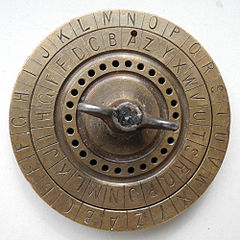
\includegraphics[width=\linewidth]{../chapter00/CaesarCipher.jpg}
		\caption[Caesar cipher]{Caesar cipher. Each letter is replaced by another one which is a fixed number of letters away from the original one. \licensequote{\cite{Berberich2013}}{Hubert Berberich}{Public Domain}}
	\end{figure}
\end{minipage}
\hfill
\begin{minipage}{0.45\linewidth}
	\begin{figure}[H]
		\centering
		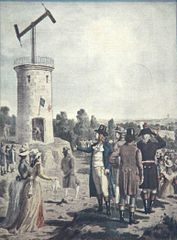
\includegraphics[width=\linewidth]{../chapter00/OpticalTelegraph.jpg}
		\caption[Optical telegraph]{Optical telegraph \cite{WikiSemaphore}}
	\end{figure}
\end{minipage}

The research of electricity created the foundations for modern communication systems. Electrical telegraphy speeded up telecommunication. At the end of the 19th century, electromagnetic waves have been discovered. James Clerk Maxwell postulated them in 1865. Heinrich Hertz produced the first electromagnetic waves in 1887. The potential had soon been acknowledged by inventors, who developed first radios. The era of analogue radio communication began. The \index{vacuum tube} vacuum tube became an important component in radio electronics.

In 1947, the bipolar transistor had been invented. This marked the beginning of the semiconductor era, which still endures. Over the decades, semiconductors became more integrated. In 1958, the first \ac{IC} had been demonstrated by Jack Kilby, engineer at Texas Instruments. At this time, wireless communication was mostly restricted to broadcasting and professional users.

With the 1990s, wireless communication technologies became more and more affordable for private usage. Advancing computer since was incorporated into communication systems. Digital communication systems gained significance and started superseding analogue communication technologies.

\addcontentsline{toc}{section}{An Innovation Motor}
\section*{An Innovation Motor}

Nowadays, innovations are driven by the demand for telecommunication which especially
\begin{itemize}
	\item is fast,
	\item is reliable,
	\item is secure,
	\item has higher throughput, and
	\item reduces the cost.
\end{itemize}

Speed and data rate are important measures, which are advertised by companies selling their products. For example, the entertainment industry like video-on-demand services require more bandwidth to deliver video streams of higher quality. Stock exchanges need low latency to trade securities within milliseconds.

Reliability is a key requirement for critical infrastructure. An unreliable system may result in loss of production or may even lead to serious dangers for health and life of people. For example, railroad traffic management requires extremely reliable communication systems for high-speed trains to prevent accidents. This goes along with security. Unauthorized parties shall have no access to the communication system. Data integrity and privacy are important.

There is often a trade-off between different requirements. No technology can fit all requirements equally. The greatest challenge for an engineer, working on Digital Communications Systems, is finding the optimal solution, which fits the customer's wishes best.

As a general rule, cost reduction is the main argument for businesses to adapt new technologies. Other requirements must of course fit. However, technologies are unlike to be implemented if they increase the monetary costs for the user.


\addcontentsline{toc}{section}{Unlimited Possibilities}
\section*{Unlimited Possibilities}

Each interconnected electronic component is a communication system. Even if a device does not communicate with its environment, its interconnected components may exchange data with each other. This shows the significance of digital communication systems. In addition, many devices provide a digital communication interface or radio link to interconnect with other devices.

Understanding digital communication systems is of great importance in many engineering and non-engineering fields, for example:
\begin{itemize}
	\item \textbf{Automation} -- 
	\item \textbf{Medical Systems} -- 
	\item \textbf{Transport} -- railway, air traffic
	\item \textbf{Public Safety} -- 
	\item \textbf{Agriculture} -- 
	\item \textbf{Energy Sector} -- 
\end{itemize}

\printbibliography[heading=subbibliography]
\end{refsection}

\clearpage

\tableofcontents
\clearpage

\setcounter{chapter}{-1}

\chapter{Course Organization}

\section{About the Lecturer}

\begin{minipage}{0.2\linewidth}
	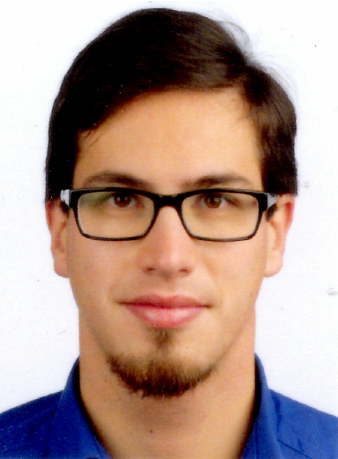
\includegraphics[width=0.8\linewidth]{../chapter00/Philipp.jpg}
\end{minipage}
\hfill
\begin{minipage}{0.75\linewidth}
	Philipp Le
	
	philipp.le@st.ovgu.de
\end{minipage}

\vspace{1em}

\underline{Academic CV:}

\begin{tabular}{p{0.2\linewidth}p{0.7\linewidth}}
	2011 -- 2015 & \makecell[l]{\textbf{B.\,Sc.} in Electrical Engineering and Information Technology,\\ Otto-von-Guericke-University Magdeburg} \\[1.5em]
	2016 & Exchange student, TU Tampere, Finland\\[0.5em]
	2015 -- 2019 & \makecell[l]{\textbf{M.\,Sc.} in Electrical Engineering and Information Technology,\\ Specialization: Communication Technology and Microwave Engineering\\ Otto-von-Guericke-University Magdeburg} \\[0.5em]
\end{tabular}

\vspace{2em}

\underline{Current occupation:}

\begin{quote}
	Since 2015: Hardware and Firmware Developer at
	
	\textbf{metraTec GmbH, Magdeburg}
	
	located in the Wissenschaftshafen.
	
	\vspace{1em}
	
	Main topics:
	\begin{itemize}
		\item Low power radio devices, IoT
		\item Radio localization
		\item Microwave engineering
	\end{itemize}
\end{quote}


\section{Course Overview}

\textit{Subject to change}

Facts on the course:
\begin{itemize}
	\item Duration: 1 semester (summer semester), 14 weeks
	\item E-Learning webpage: \url{https://elearning.ovgu.de/course/view.php?id=7849}
	\item Course material is published on the E-Learning webpage:
	\begin{itemize}
		\item Lecture notes
		\item Exercise sheets
		\item Supplementary material
	\end{itemize}
	\item Work load: 150 h (1 h = 45 minutes), yielding \textbf{5 ECTS}
	\begin{itemize}
		\item 42 h of attendance
		\item 108 h autonomous work
	\end{itemize}
	\item The research report mentioned in the module description is neglected in this semester, due to a lack of time.
	\item Written exam (120 minutes)
	\item Attending lectures or exercises not mandatory, but recommended.
\end{itemize}

Dates:
\begin{itemize}
	\item Every week: \textbf{Thursdays at 9:15 -- 10:45 (a.m.)}
	\begin{itemize}
		\item Exception: 2020-05-21 is a public holiday, no lecture! We will meet on 2020-05-19 at 15:15 -- 16:45 instead.
	\end{itemize}
	\item Additional date if necessary: Tuesdays at 15:15 -- 16:45. Will be explicitly announced on E-Learning.
	\item We will use a videoconferencing tool for our meetings. I will announce details in the E-Learning.
\end{itemize}


\section{Lecture Details}

Study organization:
\begin{itemize}
	\item You are required to elaborate major parts of the course in \underline{self-study}.
	\item The chapters of the lecture notes will be published in the E-Learning on weekly basis.
	\item Please go through the lecture notes \underline{on your own}.
	\item The lecture will be held in form of a \textbf{consultation} where we will discuss the main topics of the chapter.
	\item A pre-requisite is that you have read the lecture notes beforehand.
\end{itemize}

Remarks on the lecture notes:
\begin{itemize}
	\item The lecture notes shall give you a good foundation for your self-studies. It contains the relevant course content.
	\item If you find mistakes, don't hesitate to communicate them to me. I'm currently writing the lecture notes in nightshifts, which may lead to mistakes slipping through. ;)
\end{itemize}


\section{Exercise Details}

Goal of the exercises:
\begin{itemize}
	\item Strengthening your knowledge that you have gained in the lecture.
	\item Bringing your knowledge into action.
	\item Learning how to deal with the course material and further sources.
	\item Getting used to the nature of questions which will be asked in the exam. However, exam questions will be different.
\end{itemize}

Exercise in self-study:
\begin{itemize}
	\item Exercise sheets will be published in the E-Learning.
	\item Solve them individually or \underline{in groups}.
	\item You may ask for clarification of an exercise task at any time.
	\item \underline{You are required to put reasonable effort in solving the exercise.} This comprises referring to the lecture notes, supplementary material or other sources including the library and the internet.
	\item If you get stuck, you can contact me. I will give hints. Please be sure that you have put reasonable effort in solving beforehand.
\end{itemize}

Optional returning of solutions:
\begin{itemize}
	\item You may voluntarily return your solutions to me via E-Learning. This is not mandatory.
	\item If you wish to return your solutions, please do so within \underline{two weeks} after their publication.
	\item I will skim your solutions. Unfortunately, it is not possible for me to provide you individual corrections, as I'm lecturing besides my full time job.
	\item Of course, you may ask questions along with returning the exercises, preferably via e-mail or in the E-Learning.
	\item If I see major issues, we will discuss them together. I will integrate this into the \textbf{consultation}. The Tuesday date may be optionally used, if necessary.
	\item However, if nobody sends me a solution, we cannot discuss anything.
\end{itemize}

Please be patient if I don't answer your requests immediately. I'm giving my best to respond as soon as possible. But, I'm having a full time job which is also consuming time. :)


\section{Homework}

Your \underline{weekly} homework comprises:
\begin{itemize}
	\item Going through the lecture notes and understand its contents.
	\item If necessary, consulting further sources (library, internet) is strongly recommended.
	\item Solving the exercises.
\end{itemize}


\section{Exam Details}

\textit{All information are subject to change. There will be an announcement with details on the exam at the end of the course.}

\begin{itemize}
	\item Written exam
	\item Date: will be announced by the examination office
	\item Duration: 120 minutes
	\item Information on tools allowed will be announced at the end of the lectures.
	\item The exam covers the complete course content (all chapters, all exercise sheets).
	\item The exam questions call for different levels of skills:
	\begin{itemize}
		\item Memorized knowledge
		\item Bringing knowledge into practise
		\item Creatively deriving solutions from the knowledge
	\end{itemize}
	\item Grading scale guideline:
	\begin{itemize}
		\item 1.0 (very good): Exam performance is outstanding and goes beyond the requirements.
		\item 2.0 (good): Exam performance fulfils overall requirements.
		\item 3.0 (satisfactory): Requirements are fulfilled in general. There are minor deficiencies.
		\item 4.0 (pass): Exam performance meets the requirements, but shows major deficiencies.
		\item 5.0 (fail): Exam performance is insufficient.
	\end{itemize}
	\item Individual work. Cheating will result in a 5.0 grade (failed).
\end{itemize}


\section{Feedback Poll}

A feedback poll is required by the universities regulations for quality assurance in the teaching. Furthermore, the poll will help me to improve this course.

\textbf{So I kindly ask you to participate in the poll.}

\begin{itemize}
	\item The poll will be at the end of the course.
	\item There is an online form.
	\item The poll is completely anonymous.
	\item Participating is voluntary for you.
	\item Of course, the poll will not affect the grading. It is anonymous.
\end{itemize}

\clearpage
\phantomsection
\addcontentsline{toc}{section}{Exercise 0 - Warm Up}
\section*{Exercise 0 -- Warm Up}

Make up your mind of communication technologies and how they can be used. This exercise does not cover the actual course content, but shall give you an introduction to the topic of \emph{digital communication systems}.

\begin{question}
	Name 5 communication devices of your every-day life!
\end{question}

\begin{solution}
	\begin{itemize}
		\item Cell phone (Wifi, 4G, Bluetooth)
		\item TV
		\item PC (Wifi, Ethernet, Bluetooth)
		\item Access control key fob
		\item Bluetooth headset
	\end{itemize}
\end{solution}

\begin{question}
	Name 5 possible areas of application for digital communication systems! Describe them briefly!
\end{question}
\clearpage

\chapter{Communication Systems}

\begin{refsection}

\section{What is Communication?}

\index{communication}
\textbf{Communication} (from Latin \emph{communicare}, ``to share'') is the act of conveying information from one entity to another using mutually understood sign and symbols.

\index{information}
\textbf{Information} is the knowledge which is being conveyed from the source to the recipient. Information results in increased knowledge at the recipient's side.

Many research areas concern with communication and information:
\begin{itemize}
	\item Information theory: Quantification, storage, communication and information in general
	\item Communication studies: Human communication
	\item Linguistics: Language as a carrier of information
	\item Biosemiotics: Communication in and between living organisms
	\item ...
\end{itemize}

Communication and information are general terms. \textbf{Digital communication} concerns with the technology of conveying information using discrete signals. A \textbf{digital communication system} is a set of components and processes which implement digital communication. The signals carrying the information in a digital communication system are usually electromagnetic waves.


\section{Objectives and Distinction from Other Subjects}

This course will provide an understanding of how a digital communication system can be described. You will learn methods to describe information in their physical form as signals as well as system components. 

The theory of digital communication system is strongly connected to other subjects, for example:
\begin{itemize}
	\item Information and coding theory
	\item Computer networks
	\item Statistics
	\item Signals and systems
	\item Microwave engineering
	\item Electronics
\end{itemize}
There are courses at this university which give you a deeper insight into these subjects.


\section{Components of A Communication System}


\subsection{Communication Model}

%\todo{citation}
Claude Shannon and Warren Weaver were engineers at the Bell Telephone Labs, USA. They developed the \index{Shannon-Weaver model} \textbf{Shannon-Weaver Model} \cite{Shannon1949} (Figure \ref{fig:ch01:shannon_weaver_model}).

\begin{figure}[H]
	\centering
	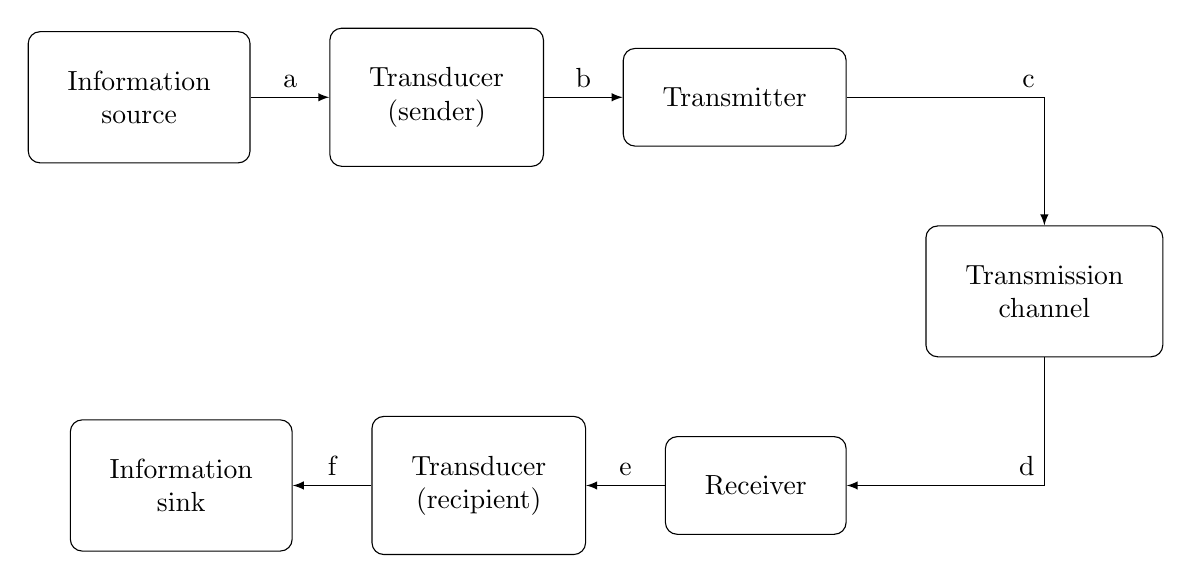
\begin{tikzpicture}
		\draw node[draw, block](Source){Information\\ source};
		\draw node[draw, block, right=of Source](STrans){Transducer\\ (sender)};
		\draw node[draw, block, right=of STrans](TX){Transmitter};
		\draw node[draw, block, below right=of TX](Ch){Transmission\\ channel};
		\draw node[draw, block, below left=of Ch](RX){Receiver};
		\draw node[draw, block, left=of RX](RTrans){Transducer\\ (recipient)};
		\draw node[draw, block, left=of RTrans](Sink){Information\\ sink};
		
		\draw[-latex] (Source) -- node[midway, align=center, above]{a} (STrans);
		\draw[-latex] (STrans) -- node[midway, align=center, above]{b} (TX);
		\draw[-latex] (TX) -| node[midway, align=center, above left]{c} (Ch);
		\draw[-latex] (Ch) |- node[midway, align=center, above left]{d} (RX);
		\draw[-latex] (RX) -- node[midway, align=center, above]{e} (RTrans);
		\draw[-latex] (RTrans) -- node[midway, align=center, above]{f} (Sink);
	\end{tikzpicture}
	\caption{Shannon-Weaver model of communication}
	\label{fig:ch01:shannon_weaver_model}
\end{figure}

\begin{description}
	\item[Information source] The information is created here.
	\item[Signal a] The original information is represented in physical form by a signal.
	\item[Transducer (sender)] The \index{Shannon-Weaver model!transducer} transducer converts the signal from one physical form to another.
	\item[Signal b] The signal is in a form which can be processed by the transmitter.
	\item[Transmitter] The information is modulated on a carrier, which can be transmitted through the transmission channel.
	\item[Signal c] The information is modulated on a carrier and can pass through the transmission channel.
	\item[Tansmission channel] The physical system through which the modulated information passes. \index{transmission channels} Transmission channels are noisy and add disturbances to the information.
	\item[Signal d] It is basically the Signal c. However, noise and disturbances have been added.
	\item[Receiver] The receiver extracts the information from the carrier. Information must be reconstructed from the noisy input signal.
	\item[Signal e] The output signal of the receiver.
	\item[Transducer (recipient)] The signal must be converted into a physical form which can be processed by the information sink.
	\item[Signal f] The signal carries the information in a form which can be used by the information sink.
	\item[Information sink] The endpoint of the information. It uses the information to gain knowledge.
\end{description}

\paragraph{Example: Cell phone}

\begin{enumerate}
	\item The information source is the brain.
	\item Electrical impulses and molecules are conveyed by the nerves to the vocal cords (transducer 1). Vocal cords convert the signals to sound.
	\item The sound is converted to an electrical signal by a microphone (transducer 2).
	\item The electrical pulses are modulated on a radio carrier (transmitter).
	\item Radio waves are transmitted over the air (transmission channel).
	\item A noisy signal is received. The receivers demodulates the information from the radio carrier.
	\item The analogue electrical signal is converted into sound by a speaker (transducer 3).
	\item The sound reaches the ear that converts them to electrical pulses (transducer 4).
	\item Electrical impulses and molecules are conveyed by the nerves to the brain (information sink).
\end{enumerate}


\subsection{Classification of Signals}

A \index{signal} signal conveys information in a form that can be processed by components of the communication systems.

\begin{figure}[H]
	\centering
	\begin{tikzpicture}
		\draw node[block](Main){\textbf{Signals carrying}\\ \textbf{information}};
		\draw node[block, below left=of Main](Analogue){Analogue};
		\draw node[block, below right=of Main](Digital){Digital};
		\draw node[block, below left=of Analogue](TimeCont){Time\\ continuous};
		\draw node[block, below right=of Analogue](TimeDis){Time\\ discrete};
		
		\draw [-latex] (Main) -- (Analogue);
		\draw [-latex] (Main) -- (Digital);
		\draw [-latex] (Analogue) -- (TimeCont);
		\draw [-latex] (Analogue) -- (TimeDis);
	\end{tikzpicture}
	\caption{Classification of signals carrying information}
	\label{fig:ch01:signals_classif}
\end{figure}

\paragraph{Analogue signals.}

\index{signal!analogue signal}
\index{signal!value-continuous}
Analogue signals are represented by values out of a continuous range (\emph{value-continuous}). The range can be limited. However, each real value in this range can be taken.

Examples:
\begin{itemize}
	\item Acoustic signals (speech, sound)
	\item Electric signals (voltage, current)
	\item Light signals (microscope, photograph)
\end{itemize}

\index{signal!time-continuous}
\index{signal!time-discrete}
Analogue signals can be time-continuous or time-discrete. \emph{Time-continuity} means that the signal is defined at any real point of time. A \emph{time-discrete} signal is only defined at certain time instances. The number of time instances can be unlimited. However, the signal is not defined between two time points.

\begin{figure}[H]
	\centering
	\begin{adjustbox}{scale=0.8}
		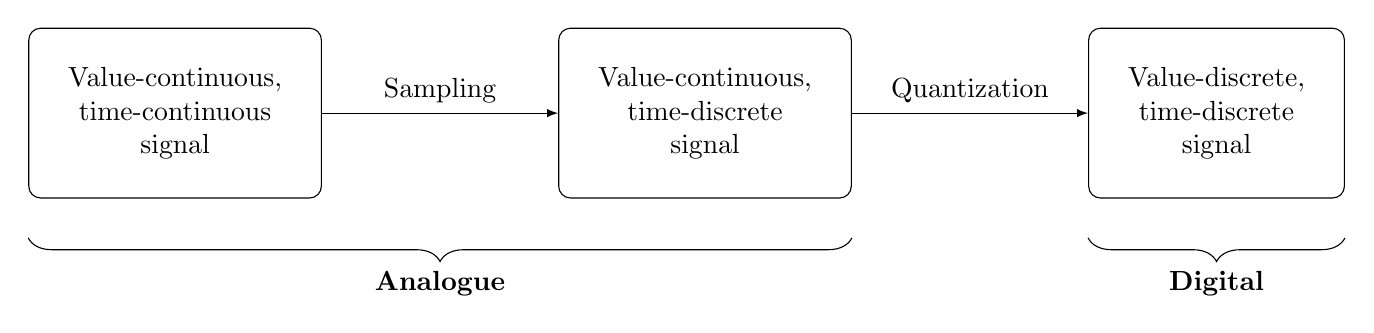
\begin{tikzpicture}
			\draw node[draw, block](Continuous){Value-continuous,\\ time-continuous\\ signal};
			\draw node[draw, block, right=3cm of Continuous](Sampled){Value-continuous,\\ time-discrete\\ signal};
			\draw node[draw, block, right=3cm of Sampled](Digital){Value-discrete,\\ time-discrete\\ signal};
			
			\draw [-latex] (Continuous) -- node[midway, align=center, above]{Sampling} (Sampled);
			\draw [-latex] (Sampled) -- node[midway, align=center, above]{Quantization} (Digital);
			
			\draw[decorate, decoration={brace, amplitude=3mm, mirror}] ([yshift=-5mm] Continuous.south west) -- ([yshift=-5mm] Sampled.south east) node[midway, below, yshift=-3mm]{\textbf{Analogue}};
			\draw[decorate, decoration={brace, amplitude=3mm, mirror}] ([yshift=-5mm] Digital.south west) -- ([yshift=-5mm] Digital.south east) node[midway, below, yshift=-3mm]{\textbf{Digital}};
		\end{tikzpicture}
	\end{adjustbox}
	\caption{Conversion from analogue to digital signals}
	\label{fig:ch01:signals_sampling}
\end{figure}

\begin{figure}[H]
	\centering
	%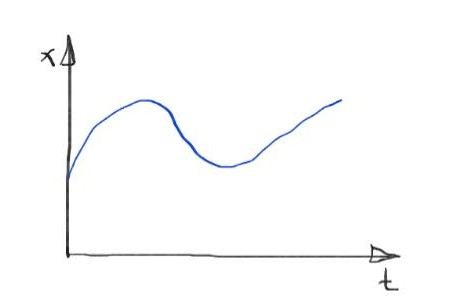
\includegraphics{../chapter01/Signal_Analogue.jpg}
	\begin{tikzpicture}
		\begin{axis}[
			height={0.25\textheight},
			width=0.6\linewidth,
			scale only axis,
			xlabel={$t$},
			ylabel={$x$},
			%grid style={line width=.6pt, color=lightgray},
			%grid=both,
			grid=none,
			axis lines=left,
			legend pos=north east,
			xmin=0,
			xmax=7,
			ymin=0,
			ymax=3,
			xtick={0, 1, ..., 6},
			ytick={0, 0.5, ..., 2.5}
		]
			\addplot[smooth, blue, thick] coordinates {(0, 1.1) (1, 1.8) (2, 2.1) (3, 1.0) (4, 0.8) (5, 1.7) (6, 2.4)};
		\end{axis}
	\end{tikzpicture}
	\caption[An analogue, value-continuous, time-continuous signal]{An analogue, value-continuous, time-continuous signal. Both time and value can be any real number.}
	\label{fig:ch01:Signal_Analogue}
\end{figure}

\begin{figure}[H]
	\centering
	%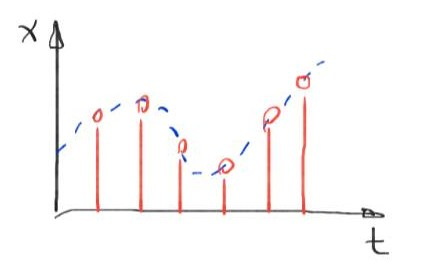
\includegraphics{../chapter01/Signal_TimeDiscr.jpg}
	\begin{tikzpicture}
		\begin{axis}[
			height={0.25\textheight},
			width=0.6\linewidth,
			scale only axis,
			xlabel={$t$},
			ylabel={$x$},
			%grid style={line width=.6pt, color=lightgray},
			%grid=both,
			grid=none,
			axis lines=left,
			legend pos=north east,
			xmin=0,
			xmax=7,
			ymin=0,
			ymax=3,
			xtick={0, 1, ..., 6},
			ytick={0, 0.5, ..., 2.5}
		]
			\addplot[smooth, blue, dashed] coordinates {(0, 1.1) (1, 1.8) (2, 2.1) (3, 1.0) (4, 0.8) (5, 1.7) (6, 2.4)};
			\addplot[red, thick] coordinates {(0, 0) (0, 1.1)};
			\addplot[red, thick] coordinates {(1, 0) (1, 1.8)};
			\addplot[red, thick] coordinates {(2, 0) (2, 2.1)};
			\addplot[red, thick] coordinates {(3, 0) (3, 1.0)};
			\addplot[red, thick] coordinates {(4, 0) (4, 0.8)};
			\addplot[red, thick] coordinates {(5, 0) (5, 1.7)};
			\addplot[red, thick] coordinates {(6, 0) (6, 2.4)};
			\addplot[only marks, red, thick, mark=o] coordinates {(0, 1.1) (1, 1.8) (2, 2.1) (3, 1.0) (4, 0.8) (5, 1.7) (6, 2.4)};
		\end{axis}
	\end{tikzpicture}
	\caption[An analogue, value-continuous, but time-discrete signal]{An analogue, value-continuous, but time-discrete signal. Only certain time points (in this case $t \in \mathbb{Z}$) are valid, but the values can be any real number. The red circles form the signal. The vertical lines illustrate that the signal in time-discrete. The blue, dashed signal is not present, but illustrates the original time-continuous signal from which the time-discrete signal has been obtained.}
	\label{fig:ch01:Signal_TimeDiscr}
\end{figure}

\paragraph{Digital signals.}

\index{signal!digital signal}
\index{signal!value-discrete}
Digital signals are both time-discrete and value-discrete. \emph{Value-discrete} means that they can take only one state out of a limited set of states.

\begin{figure}[H]
	\centering
	%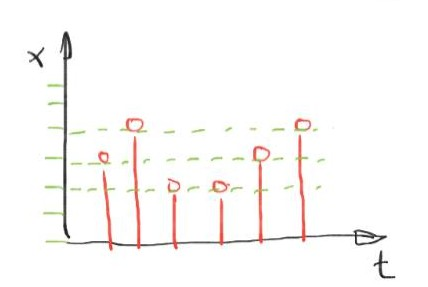
\includegraphics{../chapter01/Signal_Digital.jpg}
	\begin{tikzpicture}
		\begin{axis}[
			height={0.25\textheight},
			width=0.6\linewidth,
			scale only axis,
			xlabel={$t$},
			ylabel={$x$},
			%grid style={line width=.6pt, color=lightgray},
			%grid=both,
			xmajorgrids=false,
			ymajorgrids=true,
			grid style={color=lightgray, dashed},
			axis lines=left,
			legend pos=north east,
			xmin=0,
			xmax=7,
			ymin=0,
			ymax=3,
			xtick={0, 1, ..., 6},
			ytick={0, 0.5, ..., 2.5}
		]
			\addplot[smooth, blue, dashed] coordinates {(0, 1.1) (1, 1.8) (2, 2.1) (3, 1.0) (4, 0.8) (5, 1.7) (6, 2.4)};
			\addplot[red, thick] coordinates {(0, 0) (0, 1.0)};
			\addplot[red, thick] coordinates {(1, 0) (1, 2.0)};
			\addplot[red, thick] coordinates {(2, 0) (2, 2.0)};
			\addplot[red, thick] coordinates {(3, 0) (3, 1.0)};
			\addplot[red, thick] coordinates {(4, 0) (4, 1.0)};
			\addplot[red, thick] coordinates {(5, 0) (5, 1.5)};
			\addplot[red, thick] coordinates {(6, 0) (6, 2.5)};
			\addplot[only marks, red, thick, mark=o] coordinates {(0, 1.0) (1, 2.0) (2, 2.0) (3, 1.0) (4, 1.0) (5, 1.5) (6, 2.5)};
		\end{axis}
	\end{tikzpicture}
	\caption[A digital, value-discrete, time-discrete signal]{A digital, value-discrete, time-discrete signal. Only certain time points and a limited set of values (in this case multiples of $0.5$) are valid.}
	\label{fig:ch01:Signal_Digital}
\end{figure}

Examples:
\begin{itemize}
	\item Text letters
	\item Morse code
	\item Coded data
\end{itemize}

\index{signal!binary signal}
A special kind of digital signal is the \textbf{binary signal}. It has two discrete states.

\begin{excursus}{How analogue are digital signals?}
	In fact, the physical form of a digital signal is again an analogue signal. If digital electronics are implemented, digital signals are transferred into a physical form. A binary signal can take the discrete states ``high'' and ``low''. Being on a wire, its states are represented by voltage levels, for example \SI{0}{V} and \SI{3.3}{V}. At this point, the engineer must carefully consider the effects which the signal is subject to. This topic is covered by the field of microwave engineering and \ac{EMC}.
	
	However, if processed by a digital system, the physical representation is of minor importance. The theoretical consideration of digital signals neglects the physical nature. Even more, it is irrelevant which physical form of the digital signal exists and whether it exits. Only the discrete, logical states are of interest.
\end{excursus}


\subsection{Transmission Channels}

\index{transmission channel}
Digital communication systems employ electromagnetic waves to convey information. Therefore, only transmission channels transporting electromagnetic waves are considered.

\begin{figure}[H]
	\centering
	\begin{tikzpicture}
	\draw node[block](Main){\textbf{Transmission}\\ \textbf{channels}};
	\draw node[block, below left=of Main](Wired){Wired\\ channels};
	\draw node[block, below right=of Main](Wireless){Wireless\\ channels};
	
	\draw [-latex] (Main) -- (Wired);
	\draw [-latex] (Main) -- (Wireless);
	\end{tikzpicture}
	\caption{Classification of transmission channels}
	\label{fig:ch01:trans_ch_classif}
\end{figure}

\paragraph{Wired Channels.}

The electromagnetic wave propagates along a transmission line.

Examples of transmission lines:
\begin{itemize}
	\item Cables
	\begin{itemize}
		\item Two wire, twisted-pair \index{twisted-pair cable}
		\item Coaxial cable \index{coaxial cable}
	\end{itemize}
	\item Waveguides \index{waveguide}
	\item Planar lines (on printed circuit boards or integrated circuits)
	\begin{itemize}
		\item Microstrip \index{microstrip}
		\item Coplanar waveguide \index{coplanar waveguide}
	\end{itemize}
	\item Glass fibre (light is an electromagnetic wave, too)
\end{itemize}

\paragraph{Wireless Channels.}

The electromagnetic wave is not bound to a transmission line. It propagates through the space. A medium is not necessary. Electromagnetic wave can also travel through vacuum.

\section{The Electromagnetic Spectrum}

The carrier of information in an electronic communication system are electromagnetic waves -- either bound to a transmission line or wireless. Electromagnetic waves are electric fields $\underline{E}$ and magnetic fields $\underline{H}$, which oscillate at high frequencies.

\begin{excursus}{Maxwell's equations and wave equations}
	The Maxwell's equations are a set of coupled partial differential equations. They are the foundation of classical electromagnetism and classical optics.
	
	\textbf{Gauss' law:}
	\begin{equation}
		\nabla \cdot \cmplxvect{E} = \frac{\rho}{\varepsilon_0}
	\end{equation}
	
	\textbf{Gauss' law of magnetism:}
	\begin{equation}
		\nabla \cdot \cmplxvect{B} = 0
	\end{equation}
	
	\textbf{Faraday's law (electromagnetic induction):}
	\begin{equation}
		\nabla \times \cmplxvect{E} = - \frac{\partial \cmplxvect{B}}{\partial t}
	\end{equation}
	
	\textbf{Ampere's circuital law with Maxwell's extension:}
	\begin{equation}
		\nabla \times \cmplxvect{B} = \mu_0 \left(\cmplxvect{J} + \varepsilon_0 \frac{\partial \cmplxvect{E}}{\partial t} \right)
	\end{equation}
	
	James Clerk Maxwell postulated electromagnetic waves in 1865 \cite{Maxwell1864}. By ``decoupling'' the Maxwell's equations, the wave equations can be isolated for both the electric field and the magnetic field. They describe the wave propagation in any media.
	\begin{subequations}
		\begin{align}
			\Delta \cmplxvect{E} - \underline{\gamma}^2 \cmplxvect{E} &= \vect{0} \\
			\Delta \cmplxvect{H} - \underline{\gamma}^2 \cmplxvect{H} &= \vect{0}
		\end{align}
	\end{subequations}
	where $\underline{\gamma}$ is the complex propagation constant, that devolves into the attenuation constant $\alpha$ and the phase constant $\beta$. $\alpha$ expresses the decrease of the field amplitudes while the wave travels through a lossy medium. $\beta$ determines the propagation speed and the wavelength $\lambda = 2 \pi / \beta$.
	\begin{equation}
		\underline{\gamma} = \alpha + \mathsf{j} \beta
	\end{equation}
\end{excursus}

\begin{figure}[H]
	\centering
	\includegraphics[width=0.8\linewidth]{svg/ch01_EM_Spectrum_Properties.pdf}
	\caption{Diagram of the electromagnetic spectrum. \licensequote{\cite{Inductiveload2007}}{''Inductiveload''}{\href{https://creativecommons.org/licenses/by-sa/3.0/deed.en}{CC-BY-SA 3.0}}}
\end{figure}

Electromagnetic waves have different properties and applications, depending on the frequency. The most interesting range for communication is from radio waves to visible light.
\begin{itemize}
	\item Infrared and visible light are used in glass fibre (optical) communication systems. Before the appearance of electronic communication, light was an important information carrier (lighthouses, optical telegraphs, etc.).
	\item Radio waves and microwaves can be generated by electronics and are radiated by antennas. They have advantages over light like a wider range or their ability to penetrate walls.
\end{itemize}

Instead of the frequency, the \index{wavelength} \textbf{wavelength} $\lambda$ can be given. It is inverse proportional to the frequency with the proportionality constant $c_0$, the speed of light. The wavelength is the distance in which one period of the oscillating electromagnetic wave fits. The higher the frequency, the short the distance which a wave travels until the next period starts.
\begin{equation}
	\lambda = \frac{c_0}{f} = \frac{2 \pi c_0}{\omega}
\end{equation}

\begin{figure}[H]
	\centering
	\includegraphics[width=0.5\linewidth]{svg/ch01_Electromagnetic-Spectrum.pdf}
	\caption{Zooming into the radio spectrum as apart of the electromagnetic spectrum. \licensequote{\cite{Penubag2012}}{"Penubag" and Victor Blacus}{\href{https://creativecommons.org/licenses/by-sa/3.0/deed.en}{CC-BY-SA 3.0}}}
\end{figure}

Radio waves are used as a information carrier since the beginning of the 20th century. They can be further divided in accordance with their properties. The radio spectrum is split into \index{band} \textbf{bands}.

\renewcommand{\arraystretch}{1.5}
\begin{table}[H]
	\centering
	\caption[ITU radio band plan]{\ac{ITU} radio band plan}
	\begin{tabular}{|l|l|l|l|}
		\hline
		Band & Frequency & Properties & Example Applications \\
		\hline
		\hline
		\acs{ELF} & \SIrange{3}{30}{Hz} & \multirow{3}{*}{\begin{minipage}{0.25\textwidth}can penetrate water,\\ follows earth curvature\end{minipage}} & \multirow{3}{*}{\begin{minipage}{0.25\textwidth}submarine communication\end{minipage}} \\
		\cline{1-2}
		\acs{SLF} & \SIrange{30}{300}{Hz} &  &  \\
		\cline{1-2}
		\acs{ULF} & \SIrange{300}{3000}{Hz} &  &  \\
		\cline{1-4}
		\acs{VLF} & \SIrange{3}{30}{kHz} & \multirow{3}{*}{\begin{minipage}{0.25\textwidth}follows earth curvature\end{minipage}} & \begin{minipage}{0.25\textwidth}time signals, geophysics\end{minipage} \\[1.5em]
		\cline{1-2}
		\cline{4-4}
		\acs{LF} & \SIrange{30}{300}{kHz} &  & \begin{minipage}{0.25\textwidth}time signals, maritime navigation, AM broadcasting\end{minipage} \\[1.5em]
		\cline{1-2}
		\cline{4-4}
		\acs{MF} & \SIrange{300}{3000}{kHz} &  & \begin{minipage}{0.25\textwidth}AM broadcasting, aviation navigation, avalanche beacon\end{minipage} \\[1.5em]
		\cline{1-4}
		\acs{HF} & \SIrange{3}{30}{MHz} & \begin{minipage}{0.25\textwidth}reflections at ionosphere\end{minipage} & \begin{minipage}{0.25\textwidth}AM broadcasting, amateur radio, \acs{RFID}, maritime communication, long-distance aviation communication\end{minipage} \\[1.5em]
		\cline{1-4}
		\acs{VHF} & \SIrange{30}{300}{MHz} & \begin{minipage}{0.25\textwidth}quasi-optical propagation,\\ reflections at ionosphere possible\end{minipage} & \begin{minipage}{0.25\textwidth}FM broadcasting, television broadcasting, maritime and aviation communication, land mobile communication, weather satellites\end{minipage} \\[1.5em]
		\cline{1-4}
		\acs{UHF} & \SIrange{300}{3000}{MHz} & \multirow{3}{*}{\begin{minipage}{0.25\textwidth}quasi-optical propagation,\\ higher frequencies generally mean higher attenuation and shorter ranges\end{minipage}} & \begin{minipage}{0.25\textwidth}television broadcasting, \acs{WLAN}, \acs{GPS}, communication satellites, cell phones\end{minipage} \\[1.5em]
		\cline{1-2}
		\cline{4-4}
		\acs{SHF} & \SIrange{3}{30}{GHz} &  & \begin{minipage}{0.25\textwidth}radio astronomy, communication satellites, radar, satellite television broadcasting\end{minipage} \\[1.5em]
		\cline{1-2}
		\cline{4-4}
		\acs{EHF} & \SIrange{30}{300}{GHz} &  & \begin{minipage}{0.25\textwidth}new \acs{WLAN} standard (IEEE\,802.11ad), radar, radio astronomy, imaging (millimeter wave scanners), remote sensing\end{minipage} \\[1.5em]
		\hline
	\end{tabular}
\end{table}

Especially, the bands LF to UHF have been traditionally used in wireless communication. Furthermore, their usage is not limited to wireless systems. For example, cable television uses parts of the VHF or UHF spectra. Cable internet shares the wire with TV broadcasting.

Because of the increasing number of services and growing demands regarding bandwidth and response time, modern communication system advance in the direction of microwaves. The microwave spectrum begins at \SI{3}{GHz}.
%There are dedicate band plans for microwave applications. Table \ref{tab:ch01:IEEE_radar_bands} IEEE radar bands.

%\begin{table}[H]
%	\centering
%	\caption{IEEE radar bands}
%	\label{tab:ch01:IEEE_radar_bands}
%	\begin{tabular}{|l|}
%		\hline
%		Abbreviation \\
%		\hline
%		\hline
%		HF \\
%		\hline
%	\end{tabular}
%\end{table}

The services using the electromagnetic spectrum receive a \index{frequency allocation} \textbf{frequency allocation}. Usually, a national telecommunication regulation authority is responsible for allocation frequencies to the services. They follow recommendations of the \ac{ITU}, a special agency of the \ac{UN}. In Germany, the regulation authority is the Federal Network Agency (Bundesnetzagentur).

\section{Computer Networks}


This course focuses on the technologies which convey information between endpoints, using electromagnetic waves. The information, being conveyed, are called \textbf{data}. The handling of the data is a subject of computer science, especially \emph{computer networks} \index{computer network}. Since data processing is a part of digital communication systems, too, this digression shall give an overview about the employed concepts.


\subsection{Protocols}

Modern communication systems convey information world-wide. These communication links are established over myriads of devices, which form a network. The biggest computer network is the internet.

In order to interact, the devices are required to follow certain rules, which are called \textbf{communication protocols} \index{communication protocol}. Protocols define
\begin{itemize}
	\item the structure and semantics of data,
	\item synchronization of communication, and
	\item possible error recovery methods.
\end{itemize}

Protocols are standardized and must be implemented in every device, which interacts with other devices. Important standardization organizations are amongst others:
\begin{itemize}
	\item The non-profit organization \textbf{\acf{IETF}} issues standards concerning the internet. The standards are called \emph{Request For Comment} (RFC) and are available for everyone for free. Example standards: \ac{IP}, \ac{HTTP}
	\item The \textbf{\acf{IEEE}} has standards committees which develop and publish standards. With respect to the internet, the IEEE\,802 LAN/MAN Standards Committee is the most important one. Example standards: IEEE\,802.11 (\ac{WLAN}, Wifi)
	\item The \textbf{\acf{ETSI}} is an independent, non-profit standardization organization. It is recognized by the European Council and officially responsible for standardization of information and communication technologies in Europe. Example standards: 3G (cell phone system), 4G (cell phone system), TETRA (professional mobile radio system)
\end{itemize}


\subsection{\acs{OSI} Model}

There are many task which a digital communication systems must accomplish.
\begin{itemize}
	\item An application processes user input and displays data to the user.
	\item The application data must be reliably transferred over a network with many nodes.
	\item The network is shared with other users and applications.
	\item The network consists of many links using different physical transmission channels, for example, wired and wireless.
\end{itemize}
For each task, there are communication protocols to solve it. Communication protocols are grouped by the task which they fulfil. There is an increasing level of abstraction from the physical link to the application data. The \index{OSI model} \textbf{\acs{OSI} Model} (Figure \ref{fig:ch01:osi_model}) defines a layer structure for classifying communication protocols, which regards the level of abstraction.

\begin{figure}[H]
	\centering
	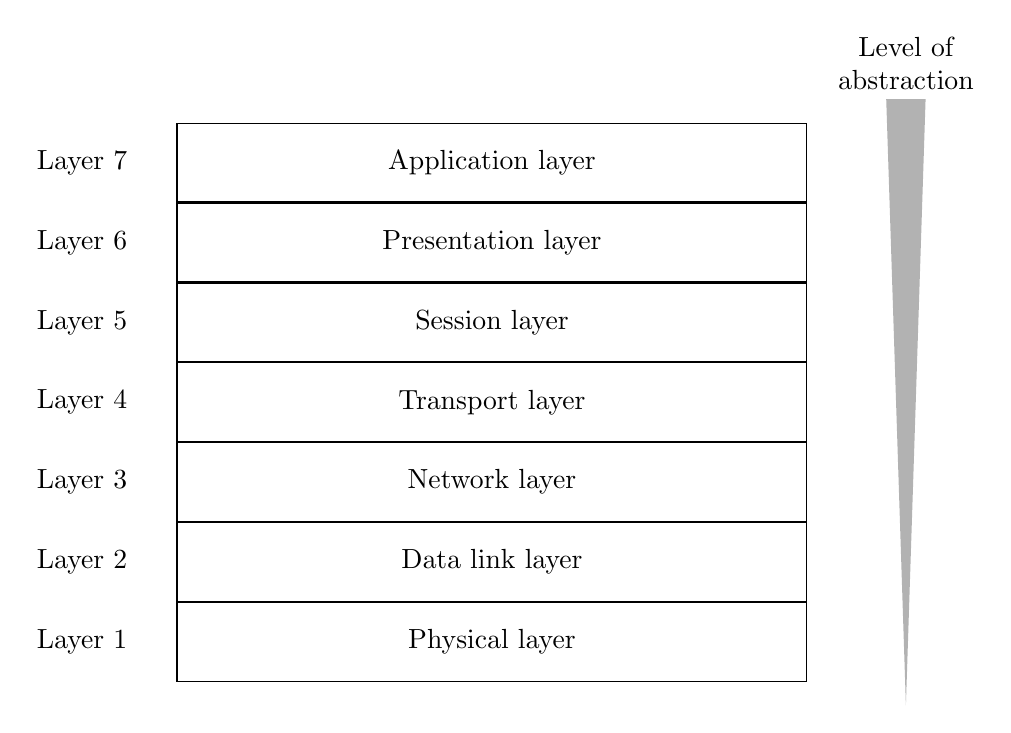
\begin{tikzpicture}[
		layer/.style={
			rectangle,
			minimum height=1cm,
			minimum width=8cm
		}
	]
		\draw node[draw, layer](L7){Application layer};
		\draw node[draw, layer, below=0 of L7](L6){Presentation layer};
		\draw node[draw, layer, below=0 of L6](L5){Session layer};
		\draw node[draw, layer, below=0 of L5](L4){Transport layer};
		\draw node[draw, layer, below=0 of L4](L3){Network layer};
		\draw node[draw, layer, below=0 of L3](L2){Data link layer};
		\draw node[draw, layer, below=0 of L2](L1){Physical layer};
		
		\node [anchor=east, align=right] at([xshift=-5mm] L7.west) {Layer 7};
		\node [anchor=east, align=right] at([xshift=-5mm] L6.west) {Layer 6};
		\node [anchor=east, align=right] at([xshift=-5mm] L5.west) {Layer 5};
		\node [anchor=east, align=right] at([xshift=-5mm] L4.west) {Layer 4};
		\node [anchor=east, align=right] at([xshift=-5mm] L3.west) {Layer 3};
		\node [anchor=east, align=right] at([xshift=-5mm] L2.west) {Layer 2};
		\node [anchor=east, align=right] at([xshift=-5mm] L1.west) {Layer 1};
		
		\filldraw[fill=gray!60, draw=none] ([xshift=10mm, yshift=3mm] L7.north east) -- node[midway, above, anchor=south, align=center]{Level of\\ abstraction} ([xshift=15mm, yshift=3mm] L7.north east) -- ([xshift=12.5mm, yshift=-3mm] L1.south east);
	\end{tikzpicture}
	\caption[OSI Model with seven layers]{\ac{OSI} Model with seven layers}
	\label{fig:ch01:osi_model}
\end{figure}

\begin{table}[H]
	\caption[Description of the layers of the OSI Model]{Description of the layers of the \ac{OSI} Model (Figure \ref{fig:ch01:osi_model}). The protocol data unit is the information }
	\begin{tabular}{|l|l|p{0.5\linewidth}|}
		\hline
		Layer & PDU & Function \\
		\hline
		\hline
		7: Application & Data & Processing user inputs, displaying data, providing services \\
		\hline
		6: Presentation & Data & Translation between network service and application (encryption, compression, etc.) \\
		\hline
		5: Session & Data & Managing sessions (retaining the communication state across multiple contacts) \\
		\hline
		4: Transport & Datagram, Segment & Reliable communication (segmentation, multiplexing, data loss detection) \\
		\hline
		3: Network & Packet & Data transfer across multiple nodes (addressing, routing, traffic control) \\
		\hline
		2: Data link & Frame & Transmission between two devices (medium access, flow control) \\
		\hline
		1: Physical & Symbol & Transmission over a physical medium \\
		\hline
	\end{tabular}
\end{table}

Each protocol has a standardized interface exposed to the upper layer, called \index{service access point} \textbf{\ac{SAP}}. They allow an upper layer protocol to execute functions of the lower layer protocol. These functions are, for example:
\begin{itemize}
	\item Sending or receiving data
	\item Control operations
	\item Network registration and de-registration
\end{itemize}

Protocol layers add own information to the data received from the upper layer. This additional information is required to provide the protocol's functionality. For example, the \acf{IP} needs to add the source and destination address, so that the packet can be routed to the correct endpoint. One can imagine this like data which is written on a letter, which is put into an envelope, which itself is put into another envelope, and so on.

\begin{figure}[H]
	\centering
	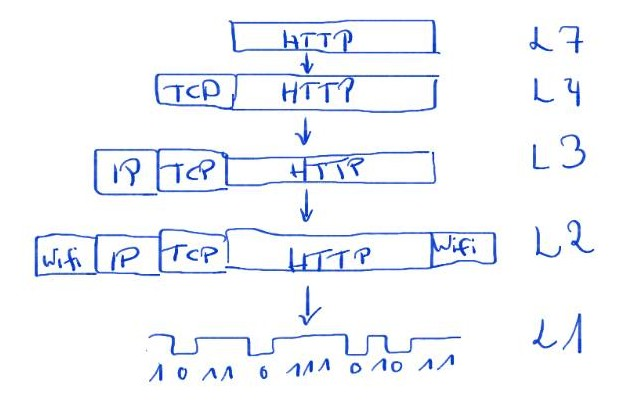
\includegraphics{../chapter01/Frame_Wrapping.jpg}
	\caption{Principle of adding more information in each protocol layer}
	\label{fig:ch01:frame_construction}
\end{figure}

Communication protocols may be exchanged in one layer without affecting the functionality of the other layers. For example, \ac{HTTP} operates on \acs{TCP}/\acs{IP}. But the \acf{IP} works on multiple physical links like Ethernet (IEEE\,802.3), Wifi (IEEE\,802.11) or 4G. The transmission media can even change along the communication path. Information travelling through the internet experience lots of \index{media change} \textbf{media changes}. For example, a datagram is firstly sent over a \ac{WLAN} link an relayed by the router on a cable to the internet service provider.


%\begin{figure}[H]
%	\centering
%	\caption{Media change on the internet. }
%	\label{fig:ch01:media_changes}
%\end{figure}

This course on digital communication systems mainly considers the physical layer (layer 1) and the data link layer (layer 2). This physical layer converts the information to physical signals which then leave the device to be transmitted over a physical transmission channel. Networks, which are enabled by protocols of layer 3 and above, are outside the scope of this course.


\subsection{Network Topologies}

In the context of networks,
\begin{itemize}
	\item the devices are called \index{node} \textbf{nodes} and
	\item the communication channels between the nodes are called \index{link} \textbf{links}.
\end{itemize}

Nodes of a network can be arranged in various ways. The structures being formed are \index{network topology} \textbf{network topologies}. Basic topologies are:
\begin{itemize}
	\item \textbf{Line} or chain -- The nodes are connected in series. A packet is passed on by each node until reaches its destination.
	\item \textbf{Ring} -- An extension of the line where the outer nodes are interconnected, too. A packet is passed by every node to its destination. The failure of a single node does not split the network into two segments, which increases the fault tolerance.
	\item \textbf{Bus} -- All nodes are connected to a central cable, the bus. Each node can receive the signals transmitted. As a drawback, only one device may occupy the bus simultaneously for transmission.
	\item \textbf{Star} -- A central node (a hub or switch) relays the packets to its destination.
	\item \textbf{Tree} -- Tree structure is a hybrid network of star networks interconnected by a bus. Because there a no loops in the network, the nodes can be graphically re-ordered to a tree graph.
	\item \textbf{Mesh} -- The nodes are interconnected directly. Nodes may have many direct connections to other nodes, while there is no hierarchy. There are many loops in the network. Usually, mesh networks are re-organized dynamically in mobile systems. A node discovers all nodes which it can reach and establishes a link. A special form is the \emph{Full Mesh}, where all nodes are interconnected with every other one.
\end{itemize}

\begin{figure}[H]
	\centering
	\includegraphics[width=0.7\linewidth]{svg/ch01_NetworkTopologies.pdf}
	\caption{Network topologies. \licensequote{\cite{Maksim2011}}{``Maksim'' and ``Malyszkz''}{Public Domain}}
\end{figure}

The network topology is a concern of the physical and data link layers of the \ac{OSI} model. It can be physical or logical.
\begin{itemize}
	\item The \index{network topology!physical topology} \textbf{physical topology} refers to the placement of the hardware. For example, in a cable network, the physical topology is defined by the cables which interconnect the devices. The topology is mainly implemented in the physical layer.
	\item The \index{network topology!logical topology} \textbf{logical topology} models the data flow in the network. For example, in a wireless network, each node can receive the signals of all other nodes in range. By addressing the devices and filtering out packets with wrong destination addresses, a logical network is created on top of the physical wireless interface. The topology is mainly implemented in the data link layer.
\end{itemize}

A network must fulfil requirements, which determine the network topology, in the end. The use case and constraints must be considered by the engineer. For example:
\begin{itemize}
	\item Lines and trees lack in reliability. The failure of one node divides the network into two segments and the remaining nodes cannot communicate with each other.
	\item The ring is an improvement of the line with respect to reliability. Lines and rings require that all nodes have equal power. Otherwise, the weakest node would be a bottleneck with respect to network bandwidth.
	\item Mesh and fully connected topologies are fault tolerant. The failure of one node does not corrupt the whole network. Furthermore, high data rates and lower latencies may be reached due to a higher number of links.
	\item Mesh and fully connected topologies increase the cost of the networks. Each link consumes energy, space and money.
	\item Buses and stars reduce the cost by maintaining a reasonable amount of reliability. The failure of one device has no major impact on the network, but a disturbance of the bus may. Buses can only be occupied by one node simultaneously. The results in lower data rate and higher latency compared to meshes.
\end{itemize}
An optimal topology may mix the basic forms.

\phantomsection
\addcontentsline{toc}{section}{References}
\printbibliography[heading=subbibliography]
\end{refsection}


\clearpage
\phantomsection
\addcontentsline{toc}{section}{Exercise 1}
\section*{Exercise 1}

\begin{question}
	What is the difference between a \emph{digital communication system} and a \emph{service}? To which OSI layers are they associated?
\end{question}
\clearpage

\chapter{Time-Continuous Signals and Systems}

\begin{refsection}

All signals considered in this chapter are \index{signal!deterministic signal} \textbf{deterministic}, i.e., its values are predictable at any time. Especially, the values can be calculated by a mathematical equation. In contrast, \emph{random} signals are not predictable. Its values are subject to a random process, which must be modelled stochastically.

\index{signal!time-continuous}
\begin{figure}[H]
	\centering
	\begin{tikzpicture}
		\draw node[block](Signals){\textbf{Signal}\\ \textbf{(deterministic)}};
		\draw node[block, below left=of Signals](Periodic){Periodic};
		\draw node[block, below right=of Signals](NonPeriodic){Non-periodic};
		\draw node[block, below left=of Periodic](Mono){Mono-chromatic};
		\draw node[block, below right=of Periodic](Multi){Multi-frequent};
		
		\draw [-latex] (Signals) -- (Periodic);
		\draw [-latex] (Signals) -- (NonPeriodic);
		\draw [-latex] (Periodic) -- (Mono);
		\draw [-latex] (Periodic) -- (Multi);
	\end{tikzpicture}
	\caption{Classification of time-continuous signals}
	\label{fig:ch02:timecont_signals_classif}
\end{figure}

\section{Mono-Chromatic Signals}

\paragraph{Representation by A Real-Valued Function.}

The mono-chromatic signal $x_{mc}(t)$ is defined by:
\begin{equation}
	x_{mc}(t) = \hat{X} \cdot \cos\left(\omega_0 t - \varphi_0\right)
	\label{eq:ch02:mono_chrom_eq}
\end{equation}
where

\begin{tabular}{ll}
	$\hat{X}$ & is the \index{amplitude} \textbf{amplitude} of the signal, \\
	$\omega_0$ & is the \index{angular frequency} \textbf{angular frequency} of the signal, \\
	$\varphi_0$ & is the \index{phase} \textbf{phase} of the signal, \\
	$t \in \mathbb{R}$ & is the real-value time variable and continuously defined.
\end{tabular}

In fact, the sine function $\sin()$ is mono-chromatic, too. However, it can be derived from \eqref{eq:ch02:mono_chrom_eq} with $\varphi_0 = \SI{90}{\degree}$.

\begin{equation*}
	x_{sin}(t) = \hat{X} \cdot \sin\left(\omega_0 t\right) = \cos\left(\omega_0 t - \SI{90}{\degree}\right)
\end{equation*}

The angular frequency is connected to the \index{frequency} \textbf{frequency}.
\begin{equation}
	\omega_0 = 2 \pi f_0
\end{equation}

\begin{attention}
	You must not confuse the terms \emph{frequency} and \emph{angular frequency}!
\end{attention}

The inverse of the frequency is the \index{period} \textbf{period} $T_0$. It is the time interval at which the signal repeats.
\begin{equation}
	T_0 = \frac{1}{f_0} = \frac{2 \pi}{\omega_0}
\end{equation}

Be aware of the units. The period $T_0$ is defined in seconds \si{s}. The frequency $f_0$ is the inverse of seconds, which is Hertz \si{Hz}. The angular frequency $\omega_0$ is the inverse of seconds, too. However, it is never given in Hertz, only in \si{rad/s} or, more commonly, \si{1/s}.

\begin{table}[H]
	\centering
	\caption{Units}
	\begin{tabular}{|l|l|}
		\hline
		Period $T_0$ & \si{s} \\
		\hline
		Frequency $f_0$ & \si{Hz} \\
		\hline
		Angular frequency $\omega_0$ & \si{1/s} \; (never Hertz!) \\
		\hline
	\end{tabular}
\end{table}

The actual unit of the signal is derived from its amplitude $\hat{X}$ which can be any physical measure.

\paragraph{Representation by A Complex-Valued Phasor.}

A graphical view on the creation of a cosine signal is depicted in Figure \ref{fig:ch02:cos_creation}.

\begin{figure}[H]
	\caption{Imagine, there is a pointer (red) with one side fixed to a point. Now, it begins rotating counter-clockwise with an angular frequency of $\omega_0$ (blue). The arrow of the pointer draws a circle (left side). Each angle of the pointer is related to a time instance (green). The blue pointer is the current position at time instance $t$. Its vertical value is projected into the time plot, forming the cosine wave (orange).}
	\label{fig:ch02:cos_creation}
\end{figure}

You may now some relations:
\begin{itemize}
	\item A full rotation of the pointer takes exactly one period $T_0$.
	\item The orange cosine curve can be horizontally shifted by redefining the original angle of the pointer at $T_0$. This offset angle is the phase $\varphi_0$.
	\item The length of the pointer and the radius of the circle is the amplitude $\hat{X}$.
\end{itemize}

A mono-chromatic signal can be described by its three parameters
\begin{itemize}
	\item Amplitude $\hat{X}$
	\item Phase $\varphi_0$
	\item Frequency $\omega_0$
\end{itemize}

When a signal passes through a \ac{LTI} system, the amplitude, the phase or both may change. However, the frequency never changes. Thus, the frequency $\omega_0$ is assumed to be constant and neglected. Consequently, the parameters
\begin{itemize}
	\item amplitude $\hat{X}$ and
	\item phase $\varphi_0$
\end{itemize}
remain. Both are absorbed by the complex-valued \index{phasor} \textbf{phasor} $\underline{X}$, which uniquely describes a mono-chromatic signal.
\begin{equation}
	\underline{X} = \hat{X} \cdot e^{-j \varphi_0} = \hat{X} \angle -\varphi_0
\end{equation}

\begin{excursus}{Complex numbers}
	$j$ is the \index{imaginary unit} \textbf{imaginary unit}. It satisfies the equation
	\begin{equation}
		j^2 = -1
	\end{equation}
	There is no real number $j \notin \mathbb{R}$ which satisfies the above solution. $j$ spans the set of complex numbers $\mathbb{C}$.
	
	In mathematics, the imaginary unit is noted as $i$. In engineering context, $j$ is used instead, because $i$ is the symbol of the electric current.
	
	A complex number $\underline{c} \in \mathbb{C}$ can be noted in \index{cartesian form} \textbf{cartesian form}:
	\begin{equation}
		\underline{c} = a + j b
	\end{equation}
	$a \in \mathbb{R}$ is the \index{real part} \textbf{real part} of $\underline{c}$. $b \in \mathbb{R}$ is the \index{imaginary part} \textbf{imaginary part} $\underline{c}$.
	\begin{subequations}
		\begin{align}
			a &= \Re\{\underline{c}\} \\
			b &= \Im\{\underline{c}\}
		\end{align}
	\end{subequations}
	Complex numbers $\underline{c}$ always carry an underline in this lecture to distinguish them from real numbers. However, this is not mandatory.

	Another notation is the \index{polar form} \textbf{polar form}:
	\begin{equation}
		\underline{c} = r \cdot e^{j \varphi}
	\end{equation}
	with
	\begin{subequations}
		\begin{align}
			r &= |\underline{c}| = \sqrt{\Re\{\underline{c}\}^2 + \Im\{\underline{c}\}^2} \\
			\varphi &= \mathrm{atan2} \left(\Im\{\underline{c}\}, \Re\{\underline{c}\}\right) \\
			e^{j \varphi} &= \cos \varphi + j \sin \varphi
		\end{align}
	\end{subequations}
	The polar form can be written in \index{angle notation} \textbf{angle notation}:
	\begin{equation}
		\underline{c} = r \angle \varphi
	\end{equation}
	$r \in \mathbb{R}$ and $\varphi \in \mathbb{R}$ are the \index{polar coordinates} \textbf{polar coordinates}.
\end{excursus}

The phasor $\underline{X} \in \mathbb{C}$ is a complex number, which is mostly represented in polar coordinates (see Figure \ref{fig:ch02:cmplxplane_phasor}).

\begin{figure}[H]
	\centering
	\begin{tikzpicture}
	\draw[->] (-3.2,0) -- (3.2,0) node[below, align=left]{$\Re$};
	\draw[->] (0,-3.2) -- (0,3.2) node[left, align=right]{$\Im$};
	\draw[->, thick] (0, 0) -- (-40:3) node[right, align=left]{Complex phasor $\underline{X}$\\ (position at $t = 0$)};
	\draw (0:1.5) arc(0:-40:1.5) node[midway, right, align=left]{Phase $\varphi_0$};
	
	\draw[->, dashed] (-50:1) arc(-50:30:1) node[right, align=left]{$\omega_0$};
	\end{tikzpicture}
	\caption{Phasor in the complex plane}
	\label{fig:ch02:cmplxplane_phasor}
\end{figure}

Figure \ref{fig:ch02:cmplxplane_phasor} depicts the phasor in the complex plane. Figure \ref{fig:ch02:cos_creation} shows a complex plane, too. Please note that both complex planes are rotated by \SI{90}{\degree} with respect to each other.

\begin{fact}
	The phasor of a signal is a signal parameter, constant and \underline{not} time-dependent.
\end{fact}

The current position of the pointer $\underline{x}(t)$ in the complex plane is obtained by rotating it. It makes a full rotation each $T_0$ periods. Therefore, it rotates at an angular frequency of $\omega_0$. The rotation is a multiplication by $e^{j \omega t}$ in the complex plane. $\underline{x}(t) \in \mathbb{C}$ is a complex value, too.
\begin{equation}
	\underline{x_{mc}}(t) = \underline{X} \cdot e^{j \omega t} = \hat{X} \cdot e^{-j \varphi_0} \cdot e^{j \omega t}
\end{equation}

\todo{Proof}

The real-valued function can be obtained by extracting the real part of the complex-valued current value.
\begin{equation}
	x_{mc}(t) = \Re\left\{\underline{x_{mc}}(t)\right\}
\end{equation}

\section{Periodic Signals and Fourier Series}

Periodic signals $x_p(t)$ comprises a class of signals which indefinitely repeat at constant time intervals $T_0$.
\begin{equation}
	x_p(t + n T_0) = x_p(t) \qquad \forall \; n \in \mathbb{Z}, \quad \mathbb{Z} = \left\{..., -2, -1, 0, 1, 2, ...\right\}
\end{equation}

Mono-chromatic signals are a special kind of periodic signals. Multi-frequent signals are composed a limited or unlimited number of mono-chromatic signals, which superimpose. Multi-frequent signals are periodic signals in general.

\begin{fact}
	Each periodic signal can be decomposed into a superposition of mono-chromatic signals.
\end{fact}

The inverse of the period $T_0$ is $f_0$, which is the \textbf{base frequency}. This is the frequency at the periodic pattern repeats. Again, frequency and angular frequency $\omega_0 = 2 \pi f_0$ must be distinguished.

The periodic signal can now be decomposed in cosine and sine functions with integer multiples of the base frequency $f_0$ or base angular frequency $\omega_0$, respectively. They are called \index{harmonics} \textbf{harmonics}.
\begin{equation}
	\begin{split}
		x_p(t) &= \sum\limits_{n=0}^{\infty} a_n \cos\left(n \omega_0 t\right) + \sum\limits_{m=0}^{\infty} b_m \sin\left(m \omega_0 t\right) \qquad \forall \; n, m \in \mathbb{N} = \left\{0, 1, 2, ...\right\} \\
		 &= a_0 + \sum\limits_{n=1}^{\infty} a_n \cos\left(n \omega_0 t\right) + \sum\limits_{m=1}^{\infty} b_m \sin\left(m \omega_0 t\right) \\
	\end{split}
	\label{eq:ch02:fourier_series}
\end{equation}

What happened to $n = 0$ and $m = 0$? $\cos(0) = 1$ and $\sin(0) = 0$. That's it.

Comparing to the mono-chromatic signals, what happened to the phase $\varphi_0$? The phase $\varphi_0$ is a characteristic of mono-chromatic signals. It is completely absorbed by the coefficients $a_n$ and $b_n$ of the cosine and sine functions.

\subsection{Orthogonality}
\index{orthogonality}
The cosine and sine functions are orthogonal to each other. In geometry, two vectors $\vect{A}$ and $\vect{B}$ are said to be orthogonal, if the angle between them is \SI{90}{\degree}. In this case, their inner product is zero.
\begin{equation}
	\langle \vect{A}, \vect{B} \rangle = 0
\end{equation}

More generally, two functions $f(x)$ and $g(x)$ are orthogonal if their \index{inner product} \textbf{inner product} $\langle f, g \rangle$ is zero. 
\begin{equation}
	0 \stackrel{!}{=} \langle f, g \rangle_w = \int\limits_{a}^{b} f(x) g(x) w(x) \, \mathrm{d} x
\end{equation}
$w(x)$ is a non-negative weight function, which is $w(x) = 1$ in simple cases like this one.

Now, you can prove that the cosine and sine functions are orthogonal to each other.
\begin{equation}
	\int\limits_{-\frac{T_0}{2}}^{\frac{T_0}{2}} \cos\left(n \omega_0 t\right) \sin\left(m \omega_0 t\right) \, \mathrm{d} t = 0 \qquad \forall \; n, m \in \mathbb{Z}
	\label{eq:ch02:orth_rel_cos_sin}
\end{equation}

Furthermore, the sine and cosine functions with \underline{different} indices are orthogonal to each other.
\begin{equation}
	\int\limits_{-\frac{T_0}{2}}^{\frac{T_0}{2}} \cos\left(n \omega_0 t\right) \cos\left(p \omega_0 t\right) \, \mathrm{d} t = \frac{\pi}{\omega_0} \cdot \delta_{np} \qquad \forall \; n, p \in \mathbb{N}
	\label{eq:ch02:orth_rel_cos}
\end{equation}
\begin{equation}
	\int\limits_{-\frac{T_0}{2}}^{\frac{T_0}{2}} \sin\left(m \omega_0 t\right) \sin\left(q \omega_0 t\right) \, \mathrm{d} t = \frac{\pi}{\omega_0} \cdot \delta_{mq} \qquad \forall \; m, q \in \mathbb{N}
	\label{eq:ch02:orth_rel_sin}
\end{equation}
with the Kronecker delta
\begin{equation}
	\delta_{uv} = \begin{cases}
		1 & \qquad \text{if } u = v, \\
		0 & \qquad \text{if } u \neq v
	\end{cases}
	\label{eq:ch02:kronecker_delta}
\end{equation}

The \index{orthogonality relations} \textbf{orthogonality relations} \eqref{eq:ch02:orth_rel_cos_sin}, \eqref{eq:ch02:orth_rel_cos} and \eqref{eq:ch02:orth_rel_sin} point out:
\begin{itemize}
	\item Cosine functions are orthogonal if their indices are different. I.e., $n \neq p$ in \eqref{eq:ch02:orth_rel_cos}.
	\item Sine functions are orthogonal if their indices are different. I.e., $m \neq q$ in \eqref{eq:ch02:orth_rel_sin}.
	\item Cosine and sine function are orthogonal independent of their indices.
	\item The indices are the integer multiples of the base frequency $\omega_0$ (harmonics).
\end{itemize}

\subsection{Extraction of The Coefficients}

The orthogonality relations are useful to extract the coefficients $a_n$ and $b_n$ in \eqref{eq:ch02:fourier_series}. Given is the input signal $\tilde{x}_p(t)$ whose coefficient shall be determined. Following assumptions can be derived from the properties of a periodic signal:
\begin{itemize}
	\item $\tilde{x}_p(t)$ is composed of mono-chromatic cosine and sine functions.
	\item All cosine and sine functions have integer multiples of the base frequency.
	\item Each cosine and sine function has a different weight -- the coefficient.
\end{itemize}

Using the orthogonality relations, the coefficients $\tilde{a}_n$ and $\tilde{b}_n$ can be obtained by:
\begin{subequations}
	\begin{align}
		\tilde{a}_n &= \frac{\omega_0}{\pi} \int\limits_{-\frac{T_0}{2}}^{\frac{T_0}{2}} \tilde{x}_p(t) \cdot \cos\left(n \omega_0 t\right) \, \mathrm{d} t \label{eq_ch02_fourier_series_coeff_an} \\
		\tilde{b}_m &= \frac{\omega_0}{\pi} \int\limits_{-\frac{T_0}{2}}^{\frac{T_0}{2}} \tilde{x}_p(t) \cdot \sin\left(n \omega_0 t\right) \, \mathrm{d} t \label{eq_ch02_fourier_series_coeff_bm}
	\end{align}
\end{subequations}

\begin{proof}{Parameter Extraction for $\tilde{a}_n$}
	Given is a periodic function $\tilde{x}_p(t)$, which can be decomposed into:
	\begin{equation}
		\tilde{x}_p(t) = \sum\limits_{p=0}^{\infty} \tilde{a}_p \cos\left(p \omega_0 t\right) + \sum\limits_{q=0}^{\infty} \tilde{b}_q \sin\left(q \omega_0 t\right)
		\label{eq_ch02_proof_per_sig_example}
	\end{equation}
	The coefficient $\tilde{a}_n$ is of interest.
	
	Inserting \eqref{eq_ch02_proof_per_sig_example} into \eqref{eq_ch02_fourier_series_coeff_an}, yields
	\begin{equation}
		\tilde{a}_n = \frac{\omega_0}{\pi} \int\limits_{-\frac{T_0}{2}}^{\frac{T_0}{2}} \left(\sum\limits_{p=0}^{\infty} \tilde{a}_p \cos\left(p \omega_0 t\right) + \sum\limits_{q=0}^{\infty} \tilde{b}_q \sin\left(q \omega_0 t\right)\right) \cdot \cos\left(n \omega_0 t\right) \, \mathrm{d} t
	\end{equation}
	Due to the orthogonality relations, \underline{all products containing a sine function} and \underline{all products containing a cosine function with the index $n \neq p$} become zero. Furthermore, following must be true: $n = p$
	
	\begin{equation}
		\tilde{a}_n = \tilde{a}_p \frac{\omega_0}{\pi} \int\limits_{-\frac{T_0}{2}}^{\frac{T_0}{2}} \cos\left(p \omega_0 t\right) \cdot \cos\left(n \omega_0 t\right) \, \mathrm{d} t \qquad \text{if } \; n = p
	\end{equation}
	
	Using \eqref{eq:ch02:orth_rel_cos}, the integral resolves to:
	\begin{equation}
		\tilde{a}_n = \tilde{a}_p \frac{\omega_0}{\pi} \frac{\pi}{\omega_0} \qquad \text{if } \; n = p
	\end{equation}
	
	In the end, it could be proven that $\tilde{a}_n = \tilde{a}_p$ for $n = p$.
	
	The proof is analogous for the coefficient $b_n$.
\end{proof}

$\cos\left(n \omega_0 t\right)$ can be seen as a ``test function'', which is used to extract the component with the index $n$. The proof points out:
\begin{itemize}
	\item All sine components are erased by $\cos\left(n \omega_0 t\right)$, due to the orthogonality relations.
	\item All cosine function with index $p \neq n$ are erased by $\cos\left(n \omega_0 t\right)$, due to the orthogonality relations.
\end{itemize}
For $b_m$, $\sin\left(m \omega_0 t\right)$ is analogous.

\begin{excursus}{Illustration of The ``Test Function''}
	For illustration of the ``test functions'', image you have a radio and want to hear a specific station. You tune to the frequency on which the station is broadcasting. All other signals are filtered out, you don't want to hear them. Actually, the radio does not employ orthogonality in this case. However, this illustration might help to understand the meaning of $\cos\left(n \omega_0 t\right)$ and $\sin\left(m \omega_0 t\right)$ \underline{in connection} with the orthogonality relations.
\end{excursus}

A special case is the coefficient $\tilde{a}_0$.
\begin{equation}
	\tilde{a}_0 = \frac{\omega_0}{\pi} \int\limits_{-\frac{T_0}{2}}^{\frac{T_0}{2}} \tilde{x}_p(t) \, \mathrm{d} t
\end{equation}
$\cos\left(n \omega_0 t\right)$ is $1$ for $n = 0$. $\tilde{a}_0$ is the \index{DC offset} \textbf{\ac{DC} offset} of the signal. The above formula is known as the calculation of the signal mean in electrical engineering.

\begin{definition}{Fourier series}
	The composition of a series of mono-chromatic signals as shown in \eqref{eq:ch02:fourier_series} is called \index{Fourier series} \textbf{Fourier series}.
	\begin{equation*}
		x_p(t) = \sum\limits_{n=1}^{\infty} a_n \cos\left(n \omega_0 t\right) + \sum\limits_{m=1}^{\infty} b_m \sin\left(m \omega_0 t\right)
	\end{equation*}
	
	The coefficients can be calculated using \eqref{eq_ch02_fourier_series_coeff_an} and \eqref{eq_ch02_fourier_series_coeff_bm}.
\end{definition}

\subsection{Complex-Valued Fourier Series}

A complex-valued, periodic signal $\underline{x_p}(t)$ can be decomposed into complex-valued mono-chromatic signals. The coefficients $\underline{c}_n$ are phasors.
\begin{equation}
	\underline{x_p}(t) = \sum\limits_{n = -\infty}^{\infty} \underline{c}_n \cdot e^{j n \omega_0 t} \qquad \forall \; n \in \mathbb{Z}
	\label{eq:ch02:fourier_series_cmplx}
\end{equation}

The coefficients $\underline{\tilde{c}}_n$ of an input signal $\underline{\tilde{x}_p}(t)$ can be determined by:
\begin{equation}
	\underline{\tilde{c}}_n = \frac{\omega_0}{2 \pi} \int\limits_{-\frac{T_0}{2}}^{\frac{T_0}{2}} \underline{\tilde{x}_p}(t) \cdot e^{-j n \omega_0 t} \, \mathrm{d} t
	\label{eq_ch02_fourier_series_coeff_cn}
\end{equation}

It is based on the orthogonality relation:
\begin{equation}
	\int\limits_{-\frac{T_0}{2}}^{\frac{T_0}{2}} e^{j n \omega_0 t} e^{-j p \omega_0 t} \, \mathrm{d} t = \frac{2 \pi}{\omega_0} \cdot \delta_{np} \qquad \forall \; n, p \in \mathbb{Z}
	\label{eq:ch02:orth_rel_exp}
\end{equation}

\begin{definition}{Complex-Valued Fourier series}
	A complex-valued, periodic signal $\underline{x_p}(t)$ can be decomposed into a series complex-valued mono-chromatic signals \eqref{eq:ch02:fourier_series_cmplx} -- the \index{Fourier series!complex-valued} \textbf{complex-valued Fourier series}.
	\begin{equation*}
		\underline{x_p}(t) = \sum\limits_{n = -\infty}^{\infty} \underline{c}_n \cdot e^{j n \omega_0 t} \qquad \forall \; n \in \mathbb{Z}
	\end{equation*}
	
	The coefficients can be calculated using \eqref{eq_ch02_fourier_series_coeff_cn}.
\end{definition}

\subsection{Amplitude and Phase Spectra}

Let's consider the complex-valued Fourier series $\underline{x_p}(t)$ \eqref{eq:ch02:fourier_series_cmplx}. The coefficients $\underline{c}_n$ are phasors. Its absolute value (amplitude) $|\underline{c}_n|$ and argument (phase) $\arg\left(\underline{c}_n\right)$ can now be plotted over the index $n$. The index $n \in \mathbb{Z}$ is discrete. Thus, the resulting plots are value-discrete in the dimension of $n$. In contrast, the amplitudes and phases are value-continuous.

\begin{definition}{Spectrum of a period signal}
	\begin{itemize}
		\item The plot of the amplitude $|\underline{c}_n|$ is called \index{amplitude spectrum} \textbf{amplitude spectrum}.
		\item The plot of the phase $\arg\left(\underline{c}_n\right)$ is called \index{phase spectrum} \textbf{phase spectrum}.
		\item When referring to the \index{spectrum} \textbf{spectrum}, generally both amplitude and phase, or their complex-valued representation of $\underline{c}_n$ is meant.
	\end{itemize}
\end{definition}

\begin{fact}
	The index $n \in \mathbb{Z}$ is discrete. The plots of the spectrum are value-discrete in the dimension of $n$.
\end{fact}

When considering a complex-valued signal $\underline{x_p}(t)$, both amplitude and phase can take any value, with following constraints:
\begin{itemize}
	\item The amplitude $|\underline{c}_n|$ is always a positive real number.
	\item The phase $\arg\left(\underline{c}_n\right)$ a real number from the interval $[-\pi, +\pi]$.
\end{itemize}

If the signal $\underline{x_p}(t) = x_p(t)$ is real-valued, i.e., $\Im\left\{\underline{c}_n(t)\right\} = 0$, the values of $\underline{c}_n$ are even more constrained by the \index{spectrum!symmetry rules} \textbf{symmetry rules}:
\begin{itemize}
	\item The coefficients $\underline{c}_n \in \mathbb{C}$ are still complex-valued phasors.
	\item But, the coefficients $\underline{c}_n$ show a special symmetry.
	\begin{itemize}
		\item The amplitude spectrum $|\underline{c}_n|$ is an \underline{even function}. It is symmetric with respect to the $y$-axis.
		\item The phase spectrum $\arg\left(\underline{c}_n\right)$ is an \underline{odd function}. It is symmetric with respect to the origin.
		\item As a consequence, the phase of $\arg\left(\underline{c}_0\right)$ at $n = 0$ must be either $0$ or $+\pi$. Note that, $+\pi$ is identical to $-\pi$ in the complex plane. Thus, $-\pi$ is valid, too, but not distinct from $+\pi$. This phase is the sign of the \ac{DC} bias: $\arg\left(\underline{c}_0\right) = 0$ means positive \ac{DC} bias and $\arg\left(\underline{c}_0\right) = \pi$ means negative \ac{DC} bias.
	\end{itemize}
\end{itemize}
These symmetry rules apply for \underline{all} real-valued signals $\underline{x_p}(t) = x_p(t) \in \mathbb{R}$. The symmetry rules ensure that the mono-chromatic components of the Fourier series \eqref{eq:ch02:fourier_series_cmplx} sum up to a real value at each time instance $t \in \mathbb{R}$.

The symmetry rules do \underline{not} apply for complex-valued signals $\underline{x_p}(t) \in \mathbb{C}$.

\begin{figure}[H]
	\centering
	\begin{tikzpicture}
		\begin{axis}[
			height={0.25\textheight},
			width=0.6\linewidth,
			scale only axis,
			xlabel={$n$},
			ylabel={$|\underline{c}_n|$},
			%grid style={line width=.6pt, color=lightgray},
			%grid=both,
			grid=none,
			axis lines=left,
			legend pos=north east,
			xmin=-4,
			xmax=4,
			ymin=0,
			ymax=3,
			xtick={-3, -2, ..., 3},
			ytick={0, 0.5, ..., 2.5},
			axis y line=middle,
			axis x line=middle,
			every axis x label/.style={
				at={(ticklabel* cs:1.05)},
				anchor=north,
			},
			every axis y label/.style={
				at={(ticklabel* cs:1.05)},
				anchor=east,
			}
		]
			\addplot[red, thick] coordinates {(-3, 0) (-3, 2.0)};
			\addplot[red, thick] coordinates {(-2, 0) (-2, 0.4)};
			\addplot[red, thick] coordinates {(-1, 0) (-1, 1.6)};
			\addplot[red, thick] coordinates {(0, 0) (0, 1.1)};
			\addplot[red, thick] coordinates {(1, 0) (1, 1.6)};
			\addplot[red, thick] coordinates {(2, 0) (2, 0.4)};
			\addplot[red, thick] coordinates {(3, 0) (3, 2.0)};
			\addplot[only marks, red, thick, mark=o] coordinates {(-3, 2.0) (-2, 0.4) (-1, 1.6) (0, 1.1) (1, 1.6) (2, 0.4) (3, 2.0)};
		\end{axis}
	\end{tikzpicture}
	\caption[Amplitude Spectrum of a multi-frequent signal]{Amplitude Spectrum of a multi-frequent signal. The absolute values (amplitudes) of the coefficients are plotted. The signal $\underline{c}_n$ is actually real-valued ($\Im\left\{\underline{c}_n(t)\right\} = 0$). This leads a symmetry with respect to the $y$-axis. The amplitude spectrum of a real-valued signal is an even function.}
	\label{fig:ch02:FSeries_Amplitude_Spectrum}
\end{figure}

\begin{figure}[H]
	\centering
	\begin{tikzpicture}
		\begin{axis}[
			height={0.25\textheight},
			width=0.6\linewidth,
			scale only axis,
			xlabel={$n$},
			ylabel={$\arg\left(\underline{c}_n\right)$},
			%grid style={line width=.6pt, color=lightgray},
			%grid=both,
			grid=none,
			axis lines=left,
			legend pos=north east,
			xmin=-4,
			xmax=4,
			ymin=-4,
			ymax=4,
			xtick={-3, -2, ..., 3},
			ytick={-3.14159, -1.5708,
1.5708, 3.14159},
			yticklabels={$-\pi\hspace{0.30cm}$, $-\frac{\pi}{2}$,
$\frac{\pi}{2}$, $\pi\hspace{0.10cm}$},
			axis y line=middle,
			axis x line=middle,
			every axis x label/.style={
				at={(ticklabel* cs:1.05)},
				anchor=north,
			},
			every axis y label/.style={
				at={(ticklabel* cs:1.05)},
				anchor=east,
			}
		]
			\addplot[red, thick] coordinates {(-3, 0) (-3, 3.14159)};
			\addplot[red, thick] coordinates {(-2, 0) (-2, -0.5)};
			\addplot[red, thick] coordinates {(-1, 0) (-1, 1.6)};
			%\addplot[red, thick] coordinates {(0, 0) (0, 0)};
			\addplot[red, thick] coordinates {(1, 0) (1, -1.6)};
			\addplot[red, thick] coordinates {(2, 0) (2, 0.5)};
			\addplot[red, thick] coordinates {(3, 0) (3, -3.14159)};
			\addplot[only marks, red, thick, mark=o] coordinates {(-3, 3.14159) (-2, -0.5) (-1, 1.6) (0, 0.0) (1, -1.6) (2, 0.5) (3, -3.14159)};
			\addplot[only marks, blue, mark=x] coordinates {(0, -3.14159) (0, 0.0) (0, 3.14159)};
		\end{axis}
	\end{tikzpicture}
	\caption[Phase Spectrum of a multi-frequent signal]{Phase Spectrum of a multi-frequent signal. The arguments (phases) of the coefficients are plotted. The signal $\underline{c}_n$ is actually real-valued ($\Im\left\{\underline{c}_n(t)\right\} = 0$). This leads a symmetry with respect to the origin. The phase spectrum of a real-valued signal is an odd function. The blue $x$ define the possible phase values of the coefficient $\underline{c}_0$ of the real-valued signal.}
	\label{fig:ch02:FSeries_Phase_Spectrum}
\end{figure}

\section{Non-Periodic Signals and Fourier Transform}

\subsection{Derivation of The Fourier Transform}

Non-periodic signals have no repeating pattern. Consequently, there is no period $T_0$. Mathematically, the period is indefinite $T_0 \rightarrow \infty$.

A non-periodic signal $\underline{x_{np}}(t)$ cannot be simply decomposed by a Fourier series \eqref{eq:ch02:fourier_series_cmplx}.
\begin{equation}
	\begin{split}
		\underline{x_{np}}(t) &= \lim\limits_{T_0 \rightarrow \infty} \sum\limits_{n = -\infty}^{\infty} \underline{c}_n \cdot e^{j n \omega_0 t} \\
		 &= \lim\limits_{T_0 \rightarrow \infty} \sum\limits_{n = -\infty}^{\infty} \underline{c}_n \cdot e^{j \frac{2 \pi n}{T_0} t}
	\end{split}
	\label{eq:ch02:sig_np_fourier_series}
\end{equation}

The coefficient $\underline{c}_n$ is defined by \eqref{eq_ch02_fourier_series_coeff_cn}:
\begin{equation*}
	\begin{split}
		\underline{c}_n &= \frac{\omega_0}{2 \pi} \int\limits_{t = -\frac{T_0}{2}}^{\frac{T_0}{2}} \underline{x_{np}}(t) \cdot e^{-j n \omega_0 t} \, \mathrm{d} t \\
		 &= \frac{1}{T_0} \int\limits_{t = -\frac{T_0}{2}}^{\frac{T_0}{2}} \underline{x_{np}}(t) \cdot e^{-j n \omega_0 t} \, \mathrm{d} t
	\end{split}
	\label{eq:ch02:sig_np_cn}
\end{equation*}

In this case where $T_0 \rightarrow \infty$, $n \omega_0$ is substituted by the frequency variable $\omega$.
\begin{equation}
	\omega = n \omega_0
	\label{eq:ch02:omega_subst}
\end{equation}

Inserting \eqref{eq:ch02:sig_np_cn} into \eqref{eq:ch02:sig_np_fourier_series} while considering \eqref{eq:ch02:omega_subst}, yields:
\begin{equation}
	\underline{x_{np}}(t) = \lim\limits_{T_0 \rightarrow \infty} \sum\limits_{n = -\infty}^{\infty} \frac{1}{T_0} \left( \int\limits_{t' = -\frac{T_0}{2}}^{\frac{T_0}{2}} \underline{x_{np}}(t') \cdot e^{-j \omega t'} \, \mathrm{d} t' \right) \cdot e^{j \omega t}
\end{equation}
Remember, that $n$ is still in the sum, since it has been absorbed by $\omega = n \omega_0$.

The outer sum is a Rieman sum. $\frac{1}{T_0}$ is substituted by $\frac{\Delta \omega}{2 \pi}$. With $T_0 \rightarrow \infty$, it can be rewritten as an integral.
\begin{equation}
	\underline{x_{np}}(t) = \underbrace{\frac{1}{2 \pi} \int\limits_{\omega = -\infty}^{\infty} \underbrace{\left( \int\limits_{t' = -\infty}^{\infty} \underline{x_{np}}(t') \cdot e^{-j \omega t'} \, \mathrm{d} t' \right)}_{\text{Fourier transform}} \cdot e^{j \omega t} \, \mathrm{d} \omega}_{\text{Inverse Fourier transform}}
\end{equation}

The inner integral is the \index{Fourier transform} \textbf{Fourier transform}. 

\begin{definition}{Fourier Transform}
	The \index{Fourier transform} \textbf{Fourier transform} of the function $\underline{x}(t)$ is:
	\begin{equation}
		\underline{X}(j \omega) = \mathcal{F} \left\{\underline{x}(t)\right\} = \int\limits_{t = -\infty}^{\infty} \underline{x}(t) \cdot e^{-j \omega t} \, \mathrm{d} t
	\end{equation}
	
	The \index{inverse Fourier transform} \textbf{inverse Fourier transform} is:
	\begin{equation}
		\underline{x}(t) = \mathcal{F}^{-1} \left\{\underline{X}(j \omega)\right\} = \frac{1}{2 \pi} \int\limits_{\omega = -\infty}^{\infty} \underline{X}(j \omega) \cdot e^{+j \omega t} \, \mathrm{d} \omega
	\end{equation}
\end{definition}

\subsection{Amplitude and Phase Spectra}

The value-continuous complex frequency variable $j \omega$ in the Fourier transforms replaced the value-discrete index $n$ of the Fourier series. Due to their similarity, the constraints for all signals and the \index{spectrum!symmetry rules} \textbf{symmetry rules} for real-valued signals apply analogously.

\begin{itemize}
	\item The Fourier transform $\underline{X}(j \omega) \in \mathbb{C}$ is always complex-valued, for both real-valued $\underline{x}(t) = x(t) \in \mathbb{R}$ and complex-valued $\underline{x}(t) \in \mathbb{C}$ signals.
	\item The amplitude $|\underline{X}(j \omega)|$ is always a positive real number.
	\item The phase $\arg\left(\underline{X}(j \omega)\right)$ a real number from the interval $[-\pi, +\pi]$.
	\item For real-valued signals $\underline{x}(t) = x(t) \in \mathbb{R}$, but not for complex-valued $\underline{x}(t) \in \mathbb{C}$ signals, following additional constraints (symmetry rules) apply:
	\begin{itemize}
		\item The amplitude spectrum $|\underline{X}(j \omega)|$ is an \underline{even function}. It is symmetric with respect to the $y$-axis.
		\item The phase spectrum $\arg\left(\underline{X}(j \omega)\right)$ is an \underline{odd function}. It is symmetric with respect to the origin.
		\item As a consequence, the phase of $\arg\left(\underline{X}(0)\right)$ at $j \omega = 0$ must be either $0$ or $+\pi$. Note that, $+\pi$ is identical to $-\pi$ in the complex plane. Thus, $-\pi$ is valid, too, but not distinct from $+\pi$. This phase is the sign of the \ac{DC} bias: $\arg\left(\underline{X}(0)\right) = 0$ means positive \ac{DC} bias and $\arg\left(\underline{X}(0)\right) = \pi$ means negative \ac{DC} bias.
	\end{itemize}
\end{itemize}

\subsection{Time Domain and Frequency Domain}

\section{Properties of The Fourier Transform}

\subsection{Energy Signals and Power Signals}

Besides the classification of signals into periodic and non-periodic, signals can be divided into \index{energy signals} \textbf{energy signals} and \index{power signals} \textbf{power signals}.

\begin{definition}{Energy and Power Signals}
	\begin{itemize}
		\item \textbf{Energy signals} have a finite, positive signal energy $0 < E < \infty$, but their average power is zero $P = 0$.
		\item \textbf{Power signals} have a finite, positive average signal power $0 < P < \infty$, but their signal energy is indefinite $E = \infty$.
	\end{itemize}
\end{definition}

The \index{average signal power} \textbf{average signal power} $P$ is a measure for the amount of energy transferred per unit time and defined by:
\begin{equation}
	P = \lim\limits_{T \rightarrow \infty} \frac{1}{T} \int\limits_{-\frac{T}{2}}^{\frac{T}{2}} \left|x(t)\right|^2 \; \mathrm{d} t
\end{equation}
The signal power is connected to the \ac{RMS} value, which is often used in electrical engineering.
\begin{equation}
	\hat{x}_{RMS} = \lim\limits_{T \rightarrow \infty} \sqrt{ \frac{1}{T} \int\limits_{-\frac{T}{2}}^{\frac{T}{2}} \left|x(t)\right|^2 \; \mathrm{d} t}
\end{equation}

The \index{signal energy} \textbf{signal energy} $E$ is:
\begin{equation}
	E = \int\limits_{-\infty}^{\infty} \left|x(t)\right|^2 \; \mathrm{d} t
\end{equation}

The property of power signals, which have an indefinite signal energy, is a problem for the Fourier transform. The transform would yield an indefinite value. Thus:
\begin{fact}
	Every energy signal has a Fourier transform.
\end{fact}

Only some power signals have a Fourier transform. There are distributions which are power signals, but have a Fourier transform, too. Especially, all \emph{tempered distributions} have a Fourier transform.

\subsection{Dirac Delta Function}

An important distribution is the \index{Dirac delta function} \textbf{Dirac delta function} $\delta(t)$. The Dirac delta function is zero everywhere except at its origin, where it is an indefinitely narrow, indefinitely high pulse.
\begin{equation}
	\delta(t) = \begin{cases}
		+\infty & \qquad \text{if } t = 0, \\
		0 & \qquad \text{if } t \neq 0
	\end{cases}
	\label{eq:ch02:dirac_delta}
\end{equation}
It is constrained by
\begin{equation}
	\int\limits_{-\infty}^{\infty} \delta(t) \; \mathrm{d} t = 1
\end{equation}

\begin{attention}
	The Dirac delta function $\delta(t)$ must not be confused with the Kronecker delta \eqref{eq:ch02:kronecker_delta}. The Dirac delta function operates in continuous space $t \in \mathbb{R}$. The Kronecker delta $\delta_n$ (here one-dimensional) operates in discrete space $n \in \mathbb{Z}$.
\end{attention}

A special feature of the function is called \index{Dirac measure} \textbf{Dirac measure}.
\begin{equation}
	\int\limits_{-\infty}^{\infty} f(t) \delta(t) \; \mathrm{d} t = f(0)
	\label{eq:ch02:dirac_measure}
\end{equation}

Using the Dirac measure, the Fourier transform can be calculated:
\begin{equation}
	\mathcal{F} \left\{\delta(t)\right\} = \int\limits_{-\infty}^{\infty} \delta(t) \cdot e^{-j \omega t} \; \mathrm{d} t = 1
\end{equation}
The Fourier transform of the Dirac delta function is the frequency-independent constant $1$.

\subsection{Operations 1: Linearity}

\subsection{Operations 2: Differentiation and Integration}

\subsection{Operations 3: Multiplication}

\subsection{Operations 4: Time Shift}

\subsection{Duality}

\section{\acs{LTI} Systems}

\subsection{Transfer Function and Impulse Response}

\subsection{Convolution}

\subsection{Poles and Zeroes}

\printbibliography[heading=subbibliography]
\end{refsection}

\clearpage

%%%%%%%%%%%%%%%%%%%%%%%%%%%%%%%%%%%%%%%%%%%%%%%%%%%%%%%%%%%
% Appendix

\begin{appendix}

%\include{appendix/crlb}

\chapter{Solutions of Exercises}

\printsolutions

\end{appendix}

%%%%%%%%%%%%%%%%%%%%%%%%%%%%%%%%%%%%%%%%%%%%%%%%%%%%%%%%%%%
% Nachtrag

% References
%\bibliographystyle{unsrt}
%\bibliography{Masterarbeit}

% Notation
%\include{formales/notation}
%\newpage

% List of Symbols
%\include{formales/formelzeichen}
\newpage

% List of Block Diagram Symbols
%\include{formales/blockfigures}
\newpage

% Print default index
\phantomsection
\addcontentsline{toc}{chapter}{Index}
\printindex
\newpage

% List of Figures
\phantomsection
\addcontentsline{toc}{chapter}{\listfigurename}
\listoffigures
\newpage

% List of Tables
\phantomsection
\addcontentsline{toc}{chapter}{\listtablename}
\listoftables
\newpage

% To Do
\pagenumbering{alph}
%\listoftodos

\end{document}
